\npara This chapter shows the development outcomes and the experiment results to proof the proposed architecture.
The first section (\textit{\ref{Results-Development}}) elaborates the outcomes of implementing the architecture.
The next three sections (\textit{\ref{Results-TechniqueComparison}}, \textit{\ref{Results-Simulation}} and \textit{\ref{Results-Deployment}}) respectively shows the results of the experiments designed in the previous section (\ref{Methodology-ExperimentDesign}).

\section{Development Outcomes} \label{Results-Development}

\subsection{Smart Contracts}

\begin{figure}[htb!]
  \centering
  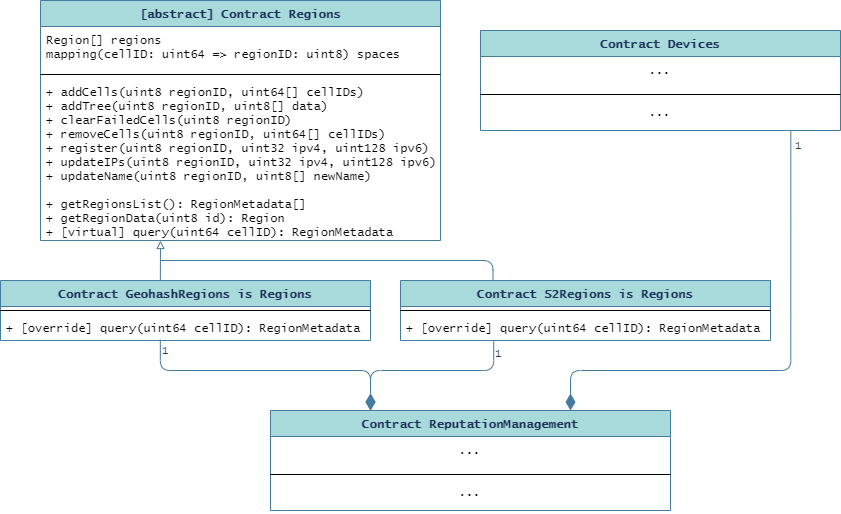
\includegraphics[width=\textwidth]{images/ContractsDeveloped.png}
  \caption{Updated \hyperref[Acronym-UML]{UML} class diagram of the Smart Contracts for supporting both geocoding techniques}
  \label{fig:ContractsDeveloped}
\end{figure}

\npara The Smart Contracts were successfully developed\footnote{GitHub repository: \url{https://github.com/ponlawat-w/uji_mt-contracts}}.
There are two different geocoding techniques, which are \textit{Geohash} and \textit{S2}.
Despite the different encoding algorithms between these two techniques, both of them result in a binary integer whose length indicates the hierarchical level of the cell.
In other words, the binary representation of the both techniques has the same structure.
Therefore, they can share the most of Smart Contract methods.

\npara Figure \ref{fig:ContractsDeveloped} shows the diagram of developed contracts.
The both geocoding techniques inherit the same abstract contract called \textit{Regions}, and they override the \textit{query} method which is the only function that they have a different behaviour, because geohash uses 5 bits to represent one level while S2 uses 2 bits.
The \code{Regions} contract was developed to be \textit{abstract}, which means that its instance cannot be initiated.
After that, the \code{Devices} contract and the \code{ReputationManagement} contract were developed.

\npara Because of that this thesis only proposes an architecture and the related technologies, so the generating of reputation value is not focused nor defined.
Therefore a direct feedback from the fog device is used in \code{ReputationManagement} contract just for proving that the contract can store and query for the value.
The practical implementation of the architecture will need to use these information of data quality and the feedback to calculate the real reputation index.

\subsection{Fog API}

\npara The \hyperref[Acronym-API]{API} for communicating with the Smart Contracts was developed\footnote{GitHub repository: \url{https://github.com/ponlawat-w/uji_mt-fog_api}}.
Each fog node serves an \hyperref[Acronym-API]{API} using the \hyperref[Acronym-HTTP]{HTTP} protocol, while it also communicates with the Geth instance through internal channel at a different port.
Therefore, the \hyperref[Acronym-API]{API} does not have to store the private key of the current node, but it can access the Blockchain through Web3 \hyperref[Acronym-API]{API} using a passphrase given by the key owner.
Through this, when a verified user wants to send a valid transaction through the fog node, the user must attach the correct passphrase in its \hyperref[Acronym-HTTP]{HTTP} request header, the \hyperref[Acronym-API]{API} will use this passphrase to decrypt the private key and unlock the account.

\npara When a user uses the \hyperref[Acronym-API]{API} to call a Smart Contract method, the \hyperref[Acronym-API]{API} needs to submit the contract call transaction to the Blockchain network, which is done by \textit{web3.js} library.
However, in some cases, it might take a longer time for the Blockchain node to mine a block and propagate the transaction.
In consequence, waiting too long for the transaction result might be interrupted by a request timeout response from the \hyperref[Acronym-HTTP]{HTTP} connection.
The user then receives an error even the transaction might be correctly pushed to the Blockchain in next few minutes.
To tackle this problem, in the developed \hyperref[Acronym-API]{API}, when a user calls a controller that submits a new transaction to the Blockchain, after \textit{web3.js} processes the request and submitted the transaction for mining, it instantly returns the transaction hash of the contract call instead of waiting until the transaction to be mined.
A user then can use the hash with another controller in the same \hyperref[Acronym-API]{API} to check the transaction status, whether it is in a queue, already mined, or rejected.

\subsection{Edge Device}

\npara The service provider and consumer code in the edge device was developed\footnote{GitHub repository: \url{https://github.com/ponlawat-w/uji_mt-edge_devices}}.
The \textit{ParticleRdWebServer} library allows a service provider to serve simple requests from its client.
Nevertheless, the usage of \textit{micro-ecc} library to sign a transaction sometimes work unexpectedly.
Even it can sign a transaction using the private key and can verify the signature by itself, but when the signature is submitted to the fog node, it is recognised to be an invalid signature.
The transaction submission request then gets rejected by the fog node and returned as a fail result.
This issue is solved by defining the number of tries to the edge device.
If the fog \hyperref[Acronym-API]{API} cannot verify the signature and responds with an error, the edge will sign and resubmit again and again until it accepts a successful response from the fog \hyperref[Acronym-API]{API}, or until it is out the number of tries.
From the observation, a transaction is usually successful between first and third try, with sometimes up to the fifth try, so the suggested number of attempts should be 5.
However, the developed code configured the number to be 10 for preparing for an unexpected case.

\subsection*{Experiment Reproducibility}

\npara The programming code, the randomly-generated input data, and the preliminary result in the experiments of this work were put into different GitHub repositories described in the footnotes.
According to \cite{Reproducibility}'s work regarding the reproducibility assessment of a research in \hyperref[Acronym-GIScience]{GIScience}, each assessment criterion can be assigned by a number between 0 and 3 which respectively means \textit{unavailable}, \textit{documented}, \textit{available}, and \textit{available and open}.
The self assignment of this work reproducibility level is by following:
\begin{itemize}
  \item \textbf{Input data:} 2
  \item \textbf{Methods preprocessing:} 2
  \item \textbf{Methods processing:} 3
  \item \textbf{Methods computational environment:} 1
  \item \textbf{Results:} 1
\end{itemize}

\newpage

\section{Experiment: Geocoding Techniques Comparison} \label{Results-TechniqueComparison}

\npara This section shows and interprets the result of two different geocoding techniques of \textit{Geohash} and \textit{S2}\footnote{GitHub repository of code in this experiment is available at\newline
\textit{Geohash: }\url{https://github.com/ponlawat-w/uji_mt-geohash_evaluation_test}\newline
\textit{S2: }\url{https://github.com/ponlawat-w/uji_mt-s2encoding}}.
However, there are some considerations regarding the bias possibility in the results as there are differences in the selected input levels of both techniques, as well as a different programming language used due to technical reasons.
This concern is elaborated in the following section (\textit{\ref{Results-TechniqueComparison-Concern}}), followed by the experiment result (\textit{\ref{Results-TechniqueComparison-Results}}).

\subsection{General Concern and Bias Consideration} \label{Results-TechniqueComparison-Concern}

\begin{table}[htb!]
  \centering
  \begin{tabular}{|c|c|r||c|c|r|}
    \hline
    \textbf{Geohash} & Bit & Cell Size & \textbf{S2} & Bit & Cell Size \\
    \hline
    1 & 5 & 12,588,175.24 km\textsuperscript{2} & 0 & 4 & 85,011,012.19 km\textsuperscript{2} \\
    & & & 1 & 6 & 21,252,753.05 km\textsuperscript{2} \\
    & & & 2 & 8 & 6,026,521.16 km\textsuperscript{2} \\
    2 & 10 & 786,760.95 km\textsuperscript{2} & 3 & 10 & 1,646,455.50 km\textsuperscript{2} \\
    & & & 4 & 12 & 413,918.15 km\textsuperscript{2} \\
    3 & 15 & 12,293.14 km\textsuperscript{2} & 5 & 14 & 104,297.91 km\textsuperscript{2} \\
    & & & 6 & 16 & 26,113.30 km\textsuperscript{2} \\
    & & & 7 & 18 & 6,529.09 km\textsuperscript{2} \\
    4 & 20 & 768.32 km\textsuperscript{2} & 8 & 20 & 1,632.45 km\textsuperscript{2} \\
    & & & 9 & 22 & 408.12 km\textsuperscript{2} \\
    5 & 25 & 12.01 km\textsuperscript{2} & 10 & 24 & 102.03 km\textsuperscript{2} \\
    & & & 11 & 26 & 25.51 km\textsuperscript{2} \\
    & & & 12 & 28 & 6.38 km\textsuperscript{2} \\
    6 & 30 & 0.75 km\textsuperscript{2} & 13 & 30 & 1.59 km\textsuperscript{2} \\
    & & & 14 & 32 & 0.40 km\textsuperscript{2} \\
    7 & 35 & 11,723.65 m\textsuperscript{2} & 15 & 34 & 99,638.93 m\textsuperscript{2} \\
    & & & 16 & 36 & 24,909.73 m\textsuperscript{2} \\
    & & & 17 & 38 & 6,227.43 m\textsuperscript{2} \\
    8 & 40 & 732.73 m\textsuperscript{2} & 18 & 40 & 1,556.86 m\textsuperscript{2} \\
    & & & 19 & 42 & 389.21 m\textsuperscript{2} \\
    & & & 20 & 44 & 97.30 m\textsuperscript{2} \\
    9 & 45 & 11.45 m\textsuperscript{2} & 21 & 46 & 24.33 m\textsuperscript{2} \\
    & & & 22 & 48 & 6.08 m\textsuperscript{2} \\
    10 & 50 & 0.72 m\textsuperscript{2} & 23 & 50 & 1.52 m\textsuperscript{2} \\
    & & & 24 & 52 & 0.38 m\textsuperscript{2} \\
    11 & 55 & 111.81 cm\textsuperscript{2} & 25 & 54 & 950.23 cm\textsuperscript{2} \\
    & & & 26 & 56 & 237.56 cm\textsuperscript{2} \\
    & & & 27 & 58 & 59.39 cm\textsuperscript{2} \\
    12 & 60 & 6.99 cm\textsuperscript{2} & 28 & 60 & 14.85 cm\textsuperscript{2} \\
    & & & 29 & 62 & 3.71 cm\textsuperscript{2} \\
    13 & 65 & 0.11 cm\textsuperscript{2} & 30 & 64 & 0.93 cm\textsuperscript{2} \\
    \hline
  \end{tabular}
  \caption{Maximum error (cell size) of different levels in Geohash and S2 Geocoding Techniques}
  \label{tab:GeohashS2Size}
\end{table}

\npara There are two issues needed to be concerned in this comparison experiment.
Firstly, the popular Geohash is based on base32 representation, despite the fact that its binary notation allows level increasing by 2 bits as S2 does, but the common Geohash libraries support only base32 manipulation.
Hence, increasing one level in a Geohash cell adds 5 more bits, but it adds 2 bits in case of S2.
The consequence is that there are no such levels where these two techniques provide a similar accuracy, and yet they cannot be fairly compared.

\npara Table \ref{tab:GeohashS2Size} shows the comparison of a cell area size between Geohash and S2 in different levels\footnote{
  \npara Geohash accuracy:\newline\href{https://stackoverflow.com/questions/13448595/geohash-string-length-and-accuracy}{\code{https://stackoverflow.com/questions/13448595/\newline
geohash-string-length-and-accuracy}}\newline
  \npara S2 cell statistics: \url{https://s2geometry.io/resources/s2cell_statistics}
}.
From the table it can be observed that at the same bit length, Geohash has a smaller cell size which means it provides more precision than S2 at the same length.
We can note that the number of S2 bits shown in the table includes the end bit of \code{1} which is insignificant for interpreting the coordinates.
For this reason, before going to compare these two techniques it needs to decide the factor for paring the levels, for example to be based on data length or cell size.
Since the Smart Contracts in this work store geocoded cells in a fixed-length integer of 64 bits, the number of bits stored is not concerned regardless of its level; therefore it compared between those levels whose area size are most similar, which are:

\begin{itemize}
  \item Geohash level 4 and S2 level 9
  \item Geohash level 5 and S2 level 12
  \item Geohash level 6 and S2 level 14
  \item Geohash level 7 and S2 level 16
\end{itemize}

Secondly, another consideration is the possible bias regarding the calculation time.
As the proposed architecture is based on JavaScript for the aforementioned reason, the library used for encoding the areas will also be developed in JavaScript.
However, there is no any S2 region covering libraries available in JavaScript library database as of found.
The official S2 library is available in C++, Go language and Python.
Go language is selected for this comparison.
This leads to the consideration that Go language is a compiled language, while JavaScript is an interpreted language; this programming language selection might affect the comparison quality.

\subsection{Comparison Results} \label{Results-TechniqueComparison-Results}

\subsubsection*{File size}

\begin{figure}[htb!]
  \centering
  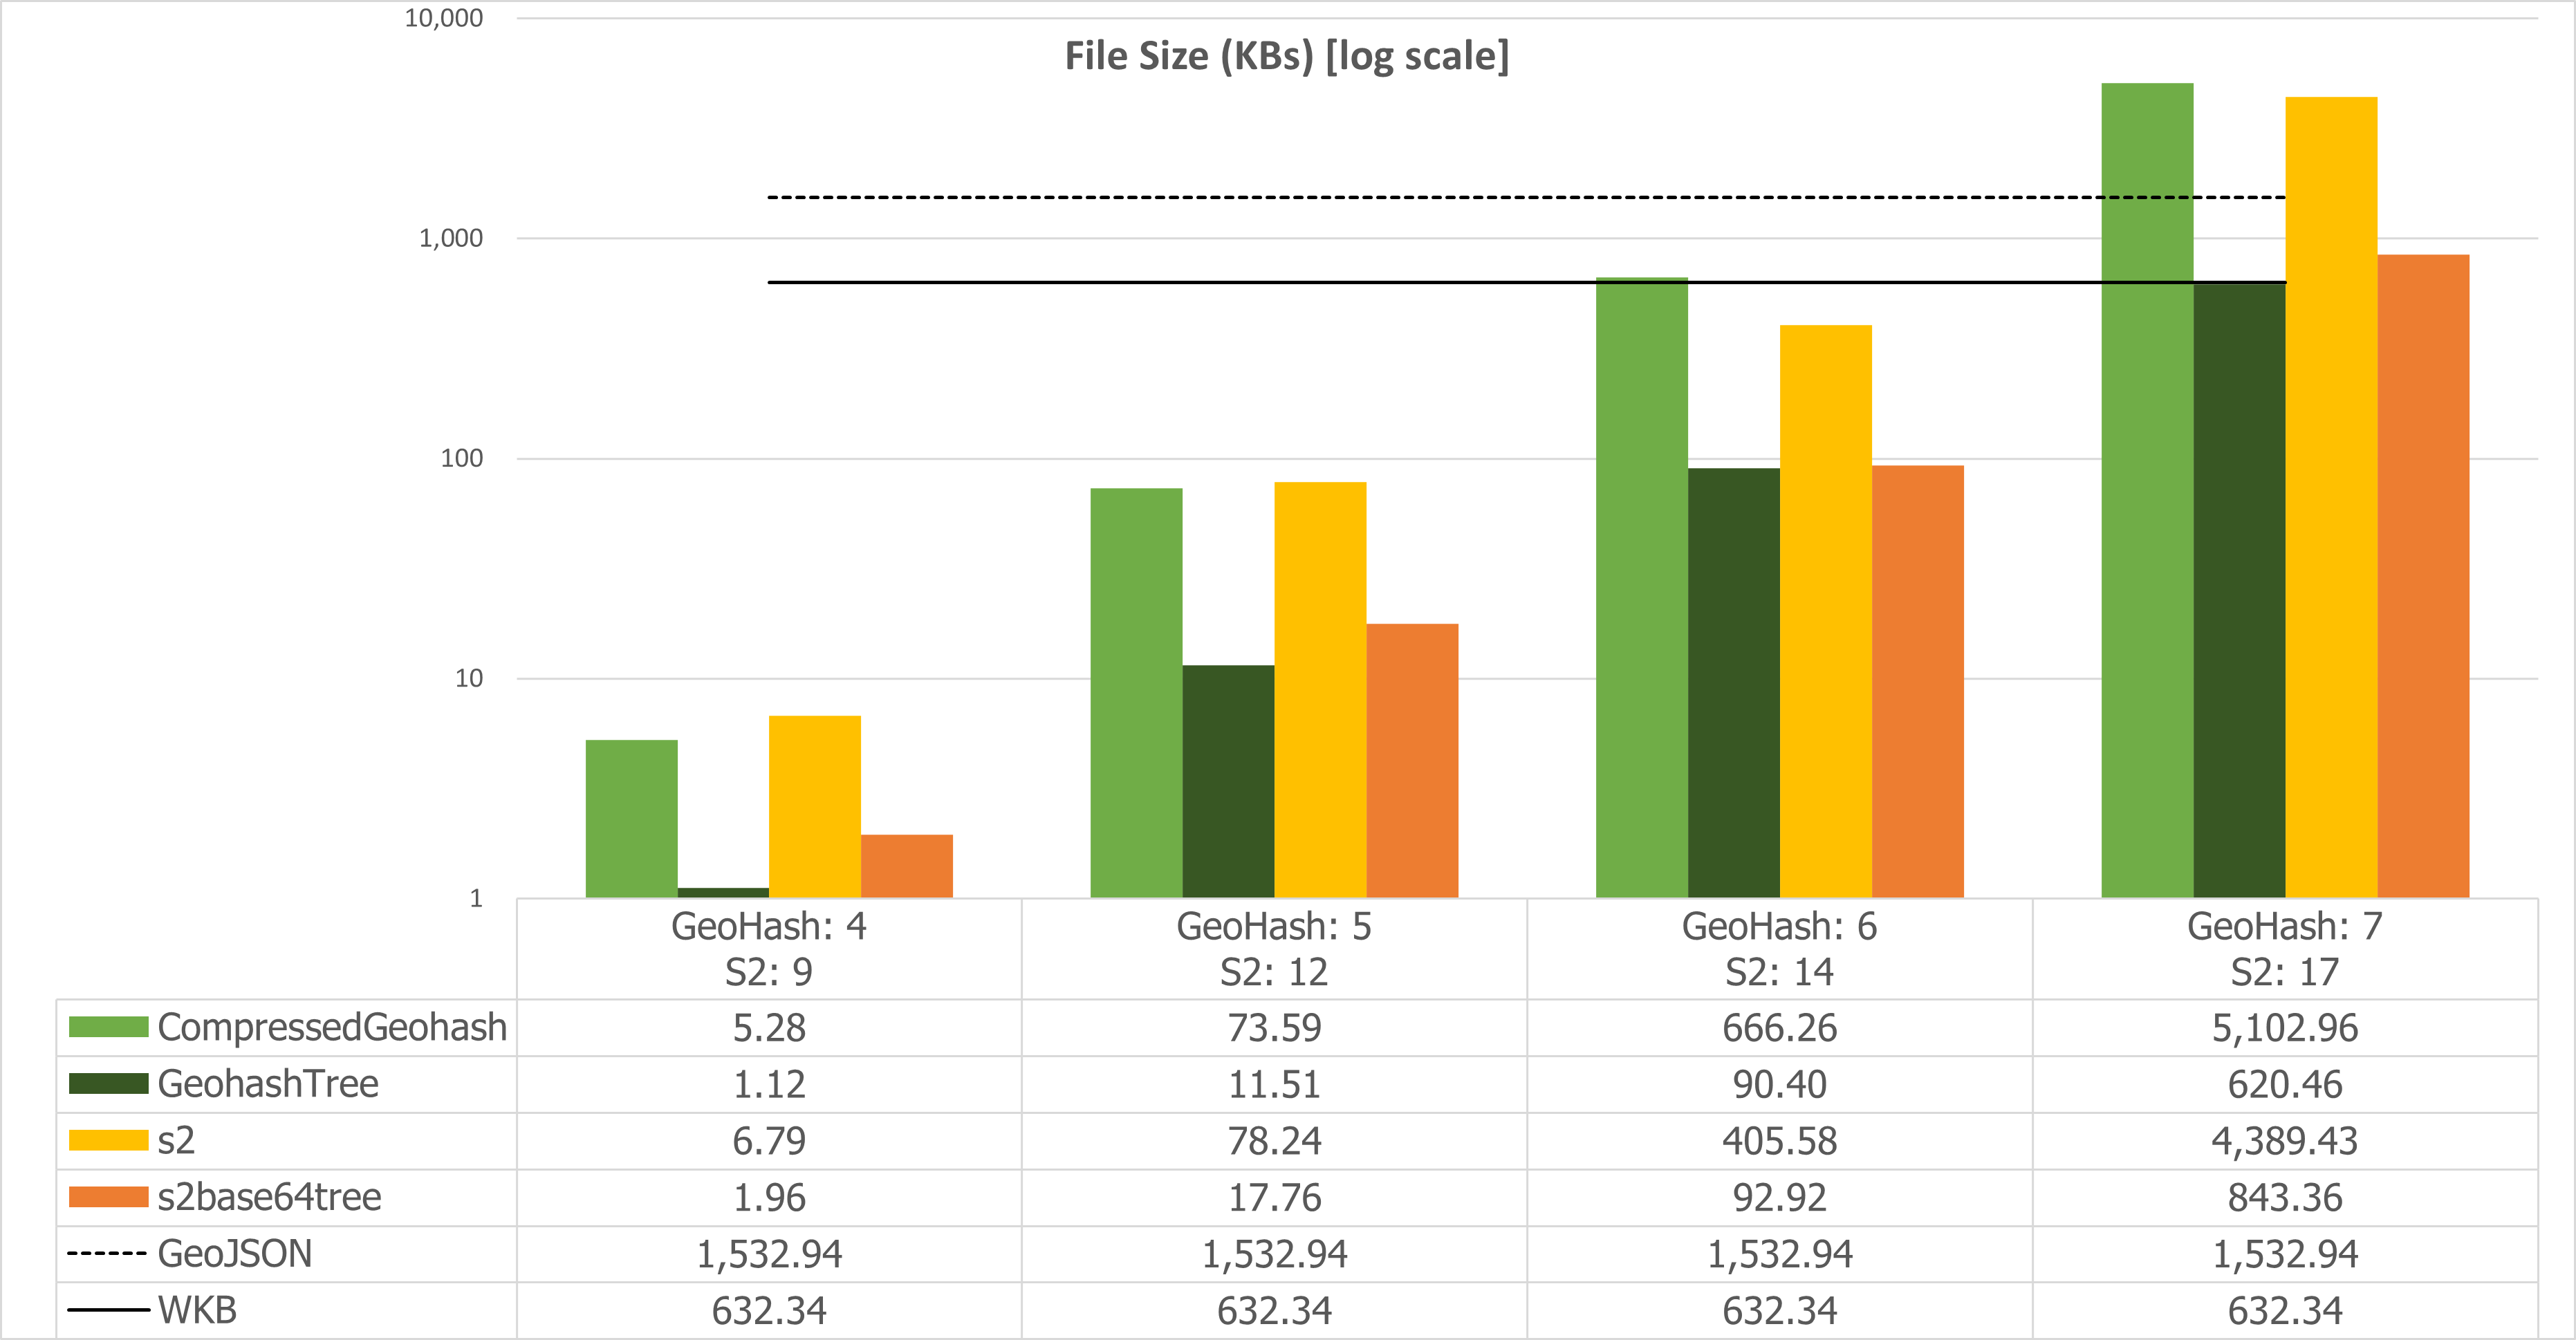
\includegraphics[width=\textwidth]{images/ResultsGSFileSize.png}
  \caption{Graph showing the file size (in kilobytes) comparison between Geohash and S2 technqiues}
  \label{fig:ResultsGSFileSize}
\end{figure}

\npara Figure \ref{fig:ResultsGSFileSize} shows the size in kilobytes of resulted geocoded cells, using the administrative region polygons in Spain as the input data.
The stable horizontal lines, black solid and dashed, are sizes of original polygons in \textit{Well-Known Binary (\hyperref[Acronym-WKB]{WKB})} and Geo\hyperref[Acronym-JSON]{JSON} respectively.
The row \code{CompressedGeohash} and \code{S2} shows the file sizes of the cell ID lists in each technique.
The row \code{GeohashTree} and \code{s2base64tree} shows the file sizes of compressed cell ID lists using the proposed algorithm.
The Graph is shown in the logarithm scale.
The result shows a very similar file size between Geohash and S2 for preserving a similar precision.
It also shows that the proposed compressing algorithm can significantly reduce the size from the prefix-redundant list.
It also demonstrates that using compressed Geohash level 6 or S2 level 14 can save disk space than the original polygonal data, but for the next level, both techniques consume a larger space than the \hyperref[Acronym-WKB]{WKB} data.

\subsubsection*{Number of Resulted Cells}

\begin{figure}[htb!]
  \centering
  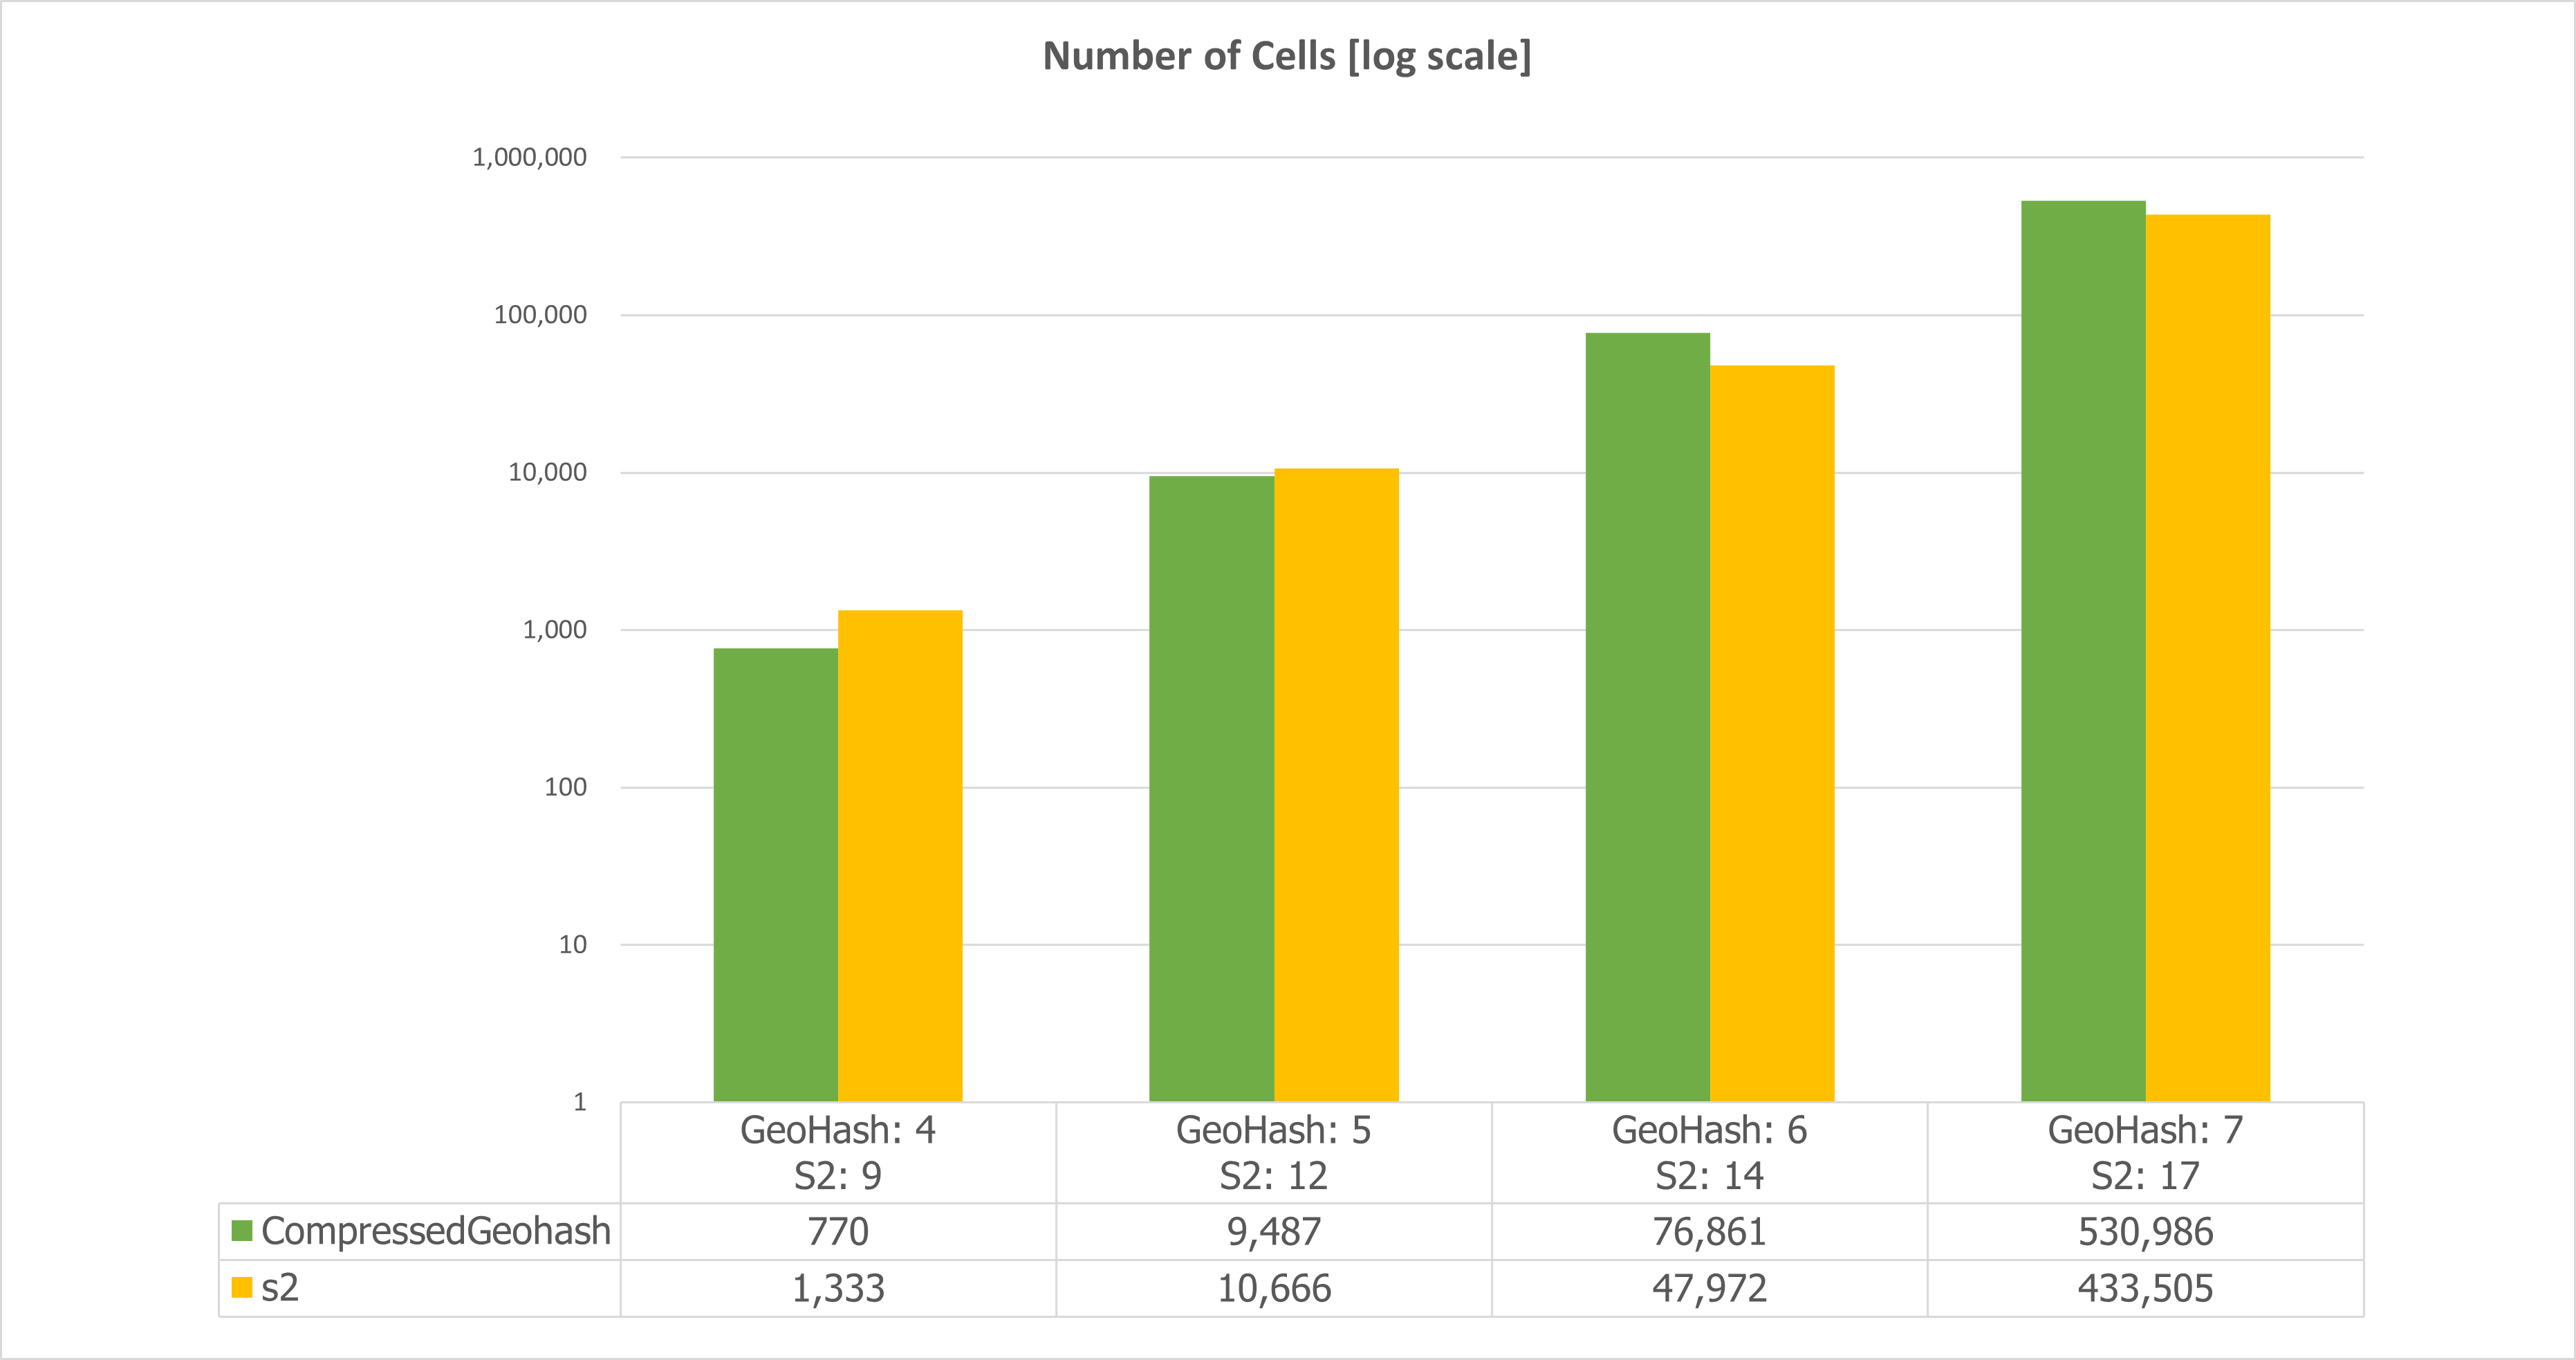
\includegraphics[width=\textwidth]{images/ResultsNumCells.png}
  \caption{Graph showing the number of cells resulted from fitting areas to geocoded cells using Geohash and S2 techniques}
  \label{fig:ResultsNumCells}
\end{figure}

\npara Figure \ref{fig:ResultsNumCells} shows the number of cells outputted from Geohash and S2 geocoding techniques.
The graph is displayed using a logarithm scale.
From the graph, it can be observed that Geohash and S2 resulted in a similar number of cells, but they are uncertain for defining which one is better, as S2 contains more number of cells in the lower level, while in the higher-level Geohash requires more.
The reason could be caused by the characteristics of the input data, such as the alignment of the input polygons.

\subsubsection*{Calculation Time}

\begin{figure}[htb!]
  \centering
  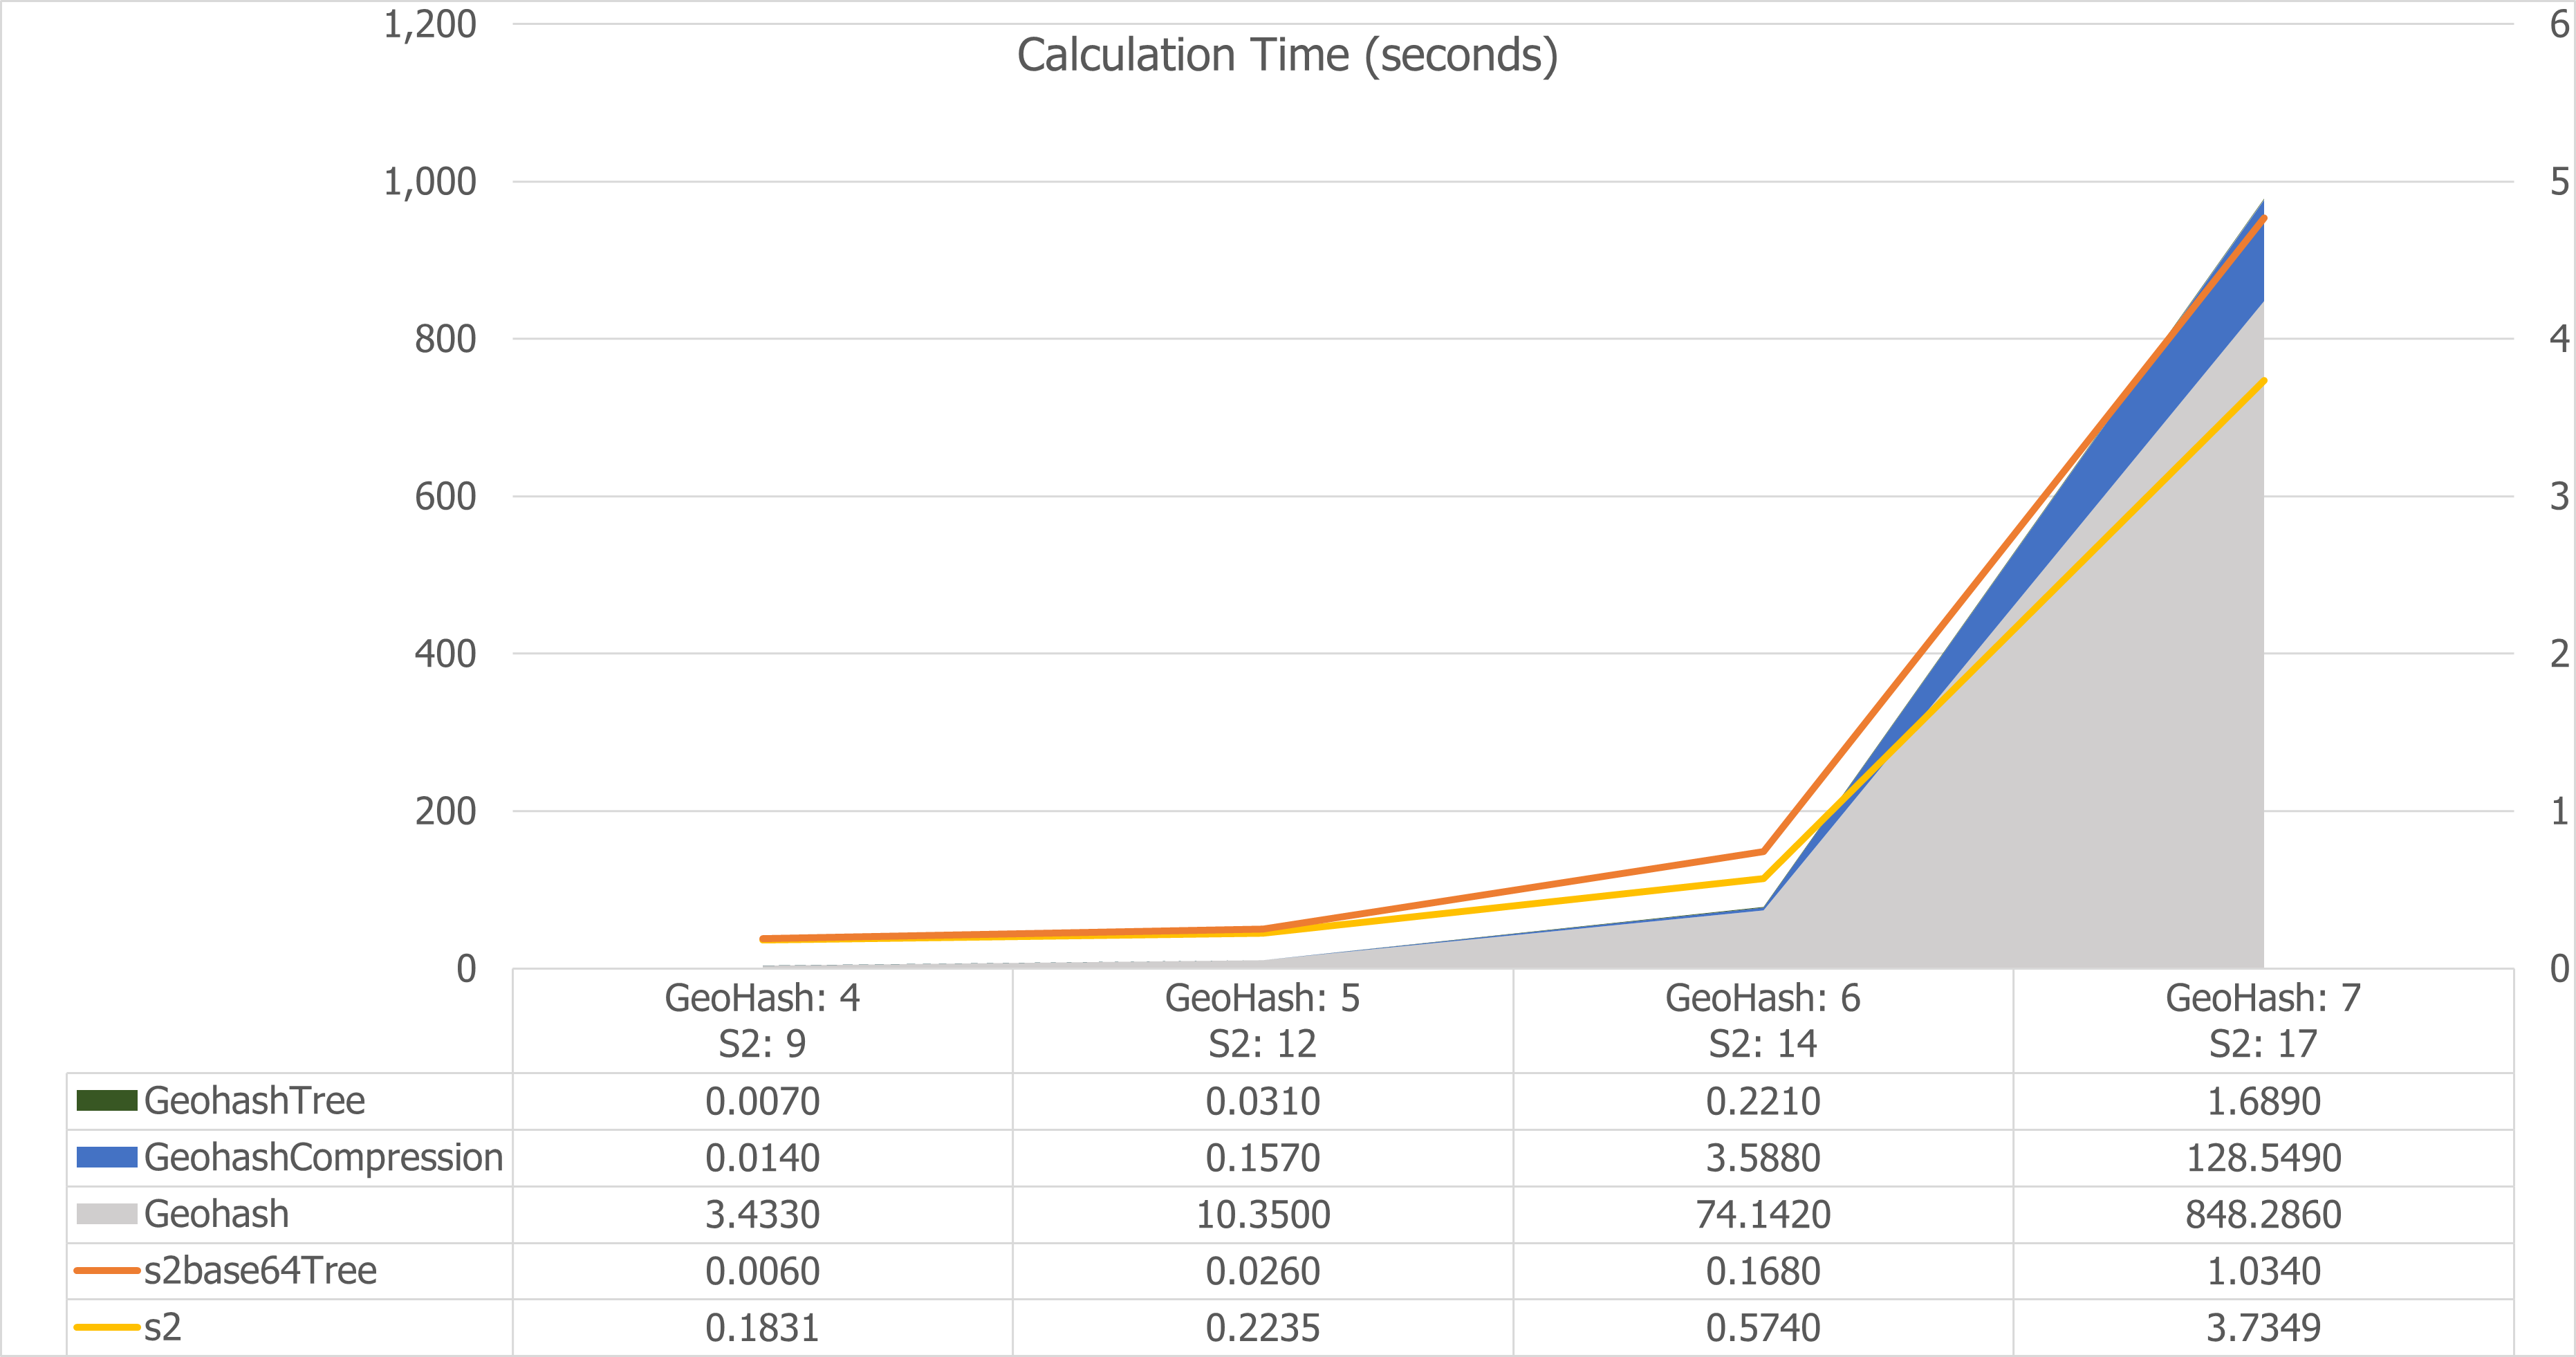
\includegraphics[width=\textwidth]{images/ResultsGSCalculationTime.png}
  \caption{Graph showing calculation time for geocoding and compressing the data using Geohash and S2 techniques}
  \label{fig:ResultsGSCalculationTime}
\end{figure}

\npara Figure \ref{fig:ResultsGSCalculationTime} shows time spent for calculation in geocoding the polygons using Geohash and S2 techniques.
The results between two techniques are too different.
The y-axis has to be split, with the left (blue) axis indicates Geohash calculation time in second, and the right (orange) indicates S2 calculation time in the same unit.
From the result, it can be observed that S2 is much faster than Geohash as converting the whole areas spent less than even 10 seconds in the highest precision, while Geohash took more than ten minutes to accomplish all the tasks.
However, the reason behind this difference could be, as described in the previous section (\textit{\ref{Results-TechniqueComparison-Concern}}), that they used a different programming language.
Furthermore, the library used for fitting the polygons into S2 cells is the official library developed by the S2 developer team, but the Geohash library is developed by a third-party developer.
\newpage

\section{Experiment: Contract Simulation} \label{Results-Simulation}

\begin{figure}[hbt!]
  \centering
  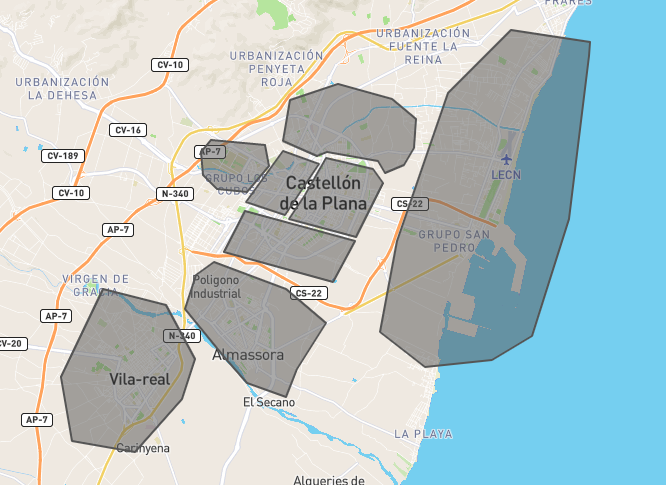
\includegraphics[width=\textwidth]{images/ExperimentInput.png}
  \caption{The region divisions of data used in the simulation experiment}
  \label{fig:ExperimentInput}
\end{figure}

\npara This section shows the simulation results of deploying the smart contracts into the Ethereum network.
There are four experiments in this section, which are 1) gas consumption in the contract deployment, 2) interacting performance with the contracts, and 3) mining performance of the devices in the system.

\npara Figure \ref{fig:ExperimentInput} shows the region divisions of data used in this experiment.
The locations used in querying and device mobility assessment in this experiment are randomly generated within these regions.

\subsection*{Gas Consumption in the Contract Deployment}

\begin{figure}[htb!]
  \centering
  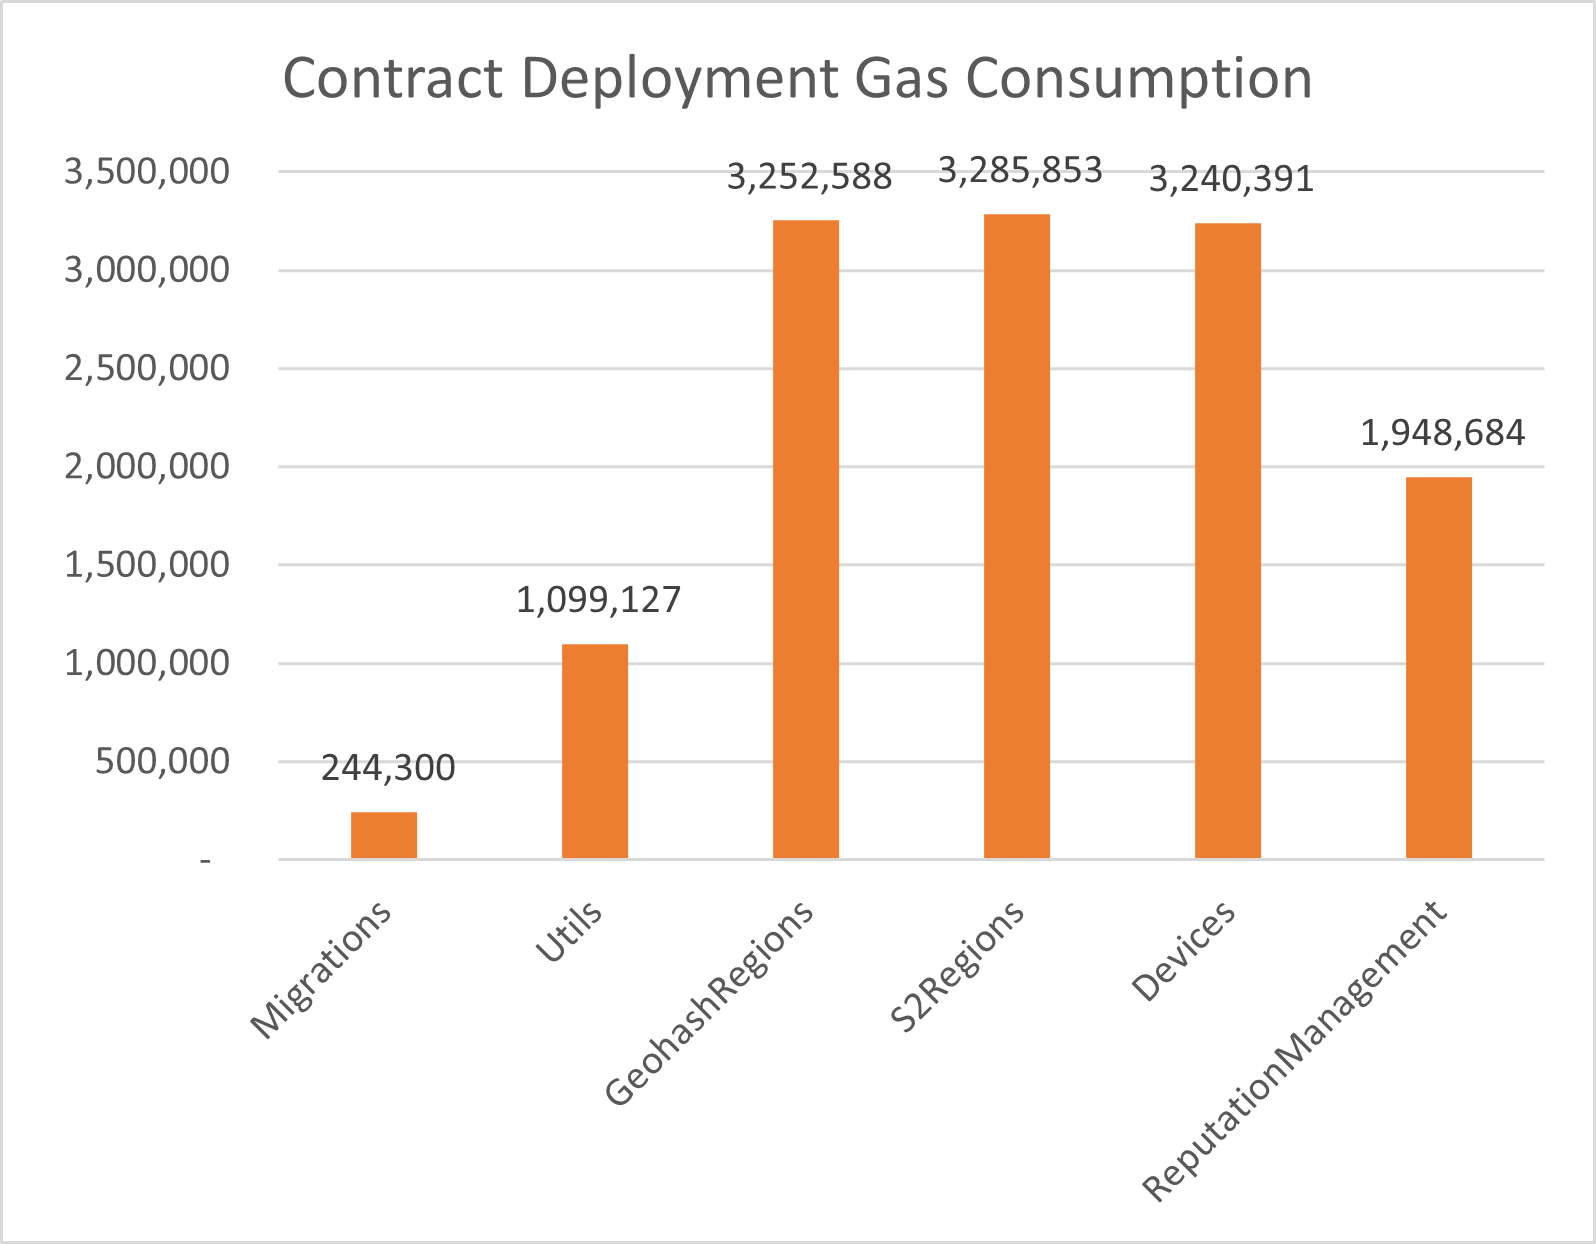
\includegraphics[width=\textwidth]{images/ExperimentDeploy.png}
  \caption{Gas consumption in contracts deployment}
  \label{fig:ExperimentDeploy}
\end{figure}

\npara This experiment measures the Ethereum gas spent on deploying the developed Smart Contracts into the Ethereum Network.
Figure \ref{fig:ExperimentDeploy} shows the result of the experiment.
From the result, it can be observed that \textit{Regions} and \textit{Devices} Contracts use more gas comparing to the other contracts.
This is caused from the number of methods and the computational operations in the contracts.
It can also be observed that the implementation of the regions based on \textit{S2} geocoding technique consumes slightly more gas than the \textit{Geohash} one.
The reason behind this difference could be that the operations in S2 have to handle the end bit of the cell when changing the level, while the action is unnecessary in Geohash.

\subsection*{Interacting Performance with the Regions Contracts}

\npara This experiment added a number of example regions data (Figure \ref{fig:ExperimentInput}) into the Smart Contracts that use Geohash and S2.
The design of this experiment divided data inputs into three different levels.
In case of Geohash, the maximum cell lengths are 6, 7, and 8.
And in case of S2, they are 14, 17, and 19.
However, the Smart Contracts returned an \textit{out of gas} error when trying to add the regions of the third level in the both techniques (Geohash: 8, S2: 19).
For this reason, this experiment results will only show the first two lengths:

\begin{itemize}
  \item \textbi{Geohash Precision 1}: 6
  \item \textbi{Geohash Precision 2}: 7
  \item \textbi{S2 Precision 1}: 14
  \item \textbi{S2 Precision 2}: 17
\end{itemize}

\begin{figure}[htb!]
  \centering
  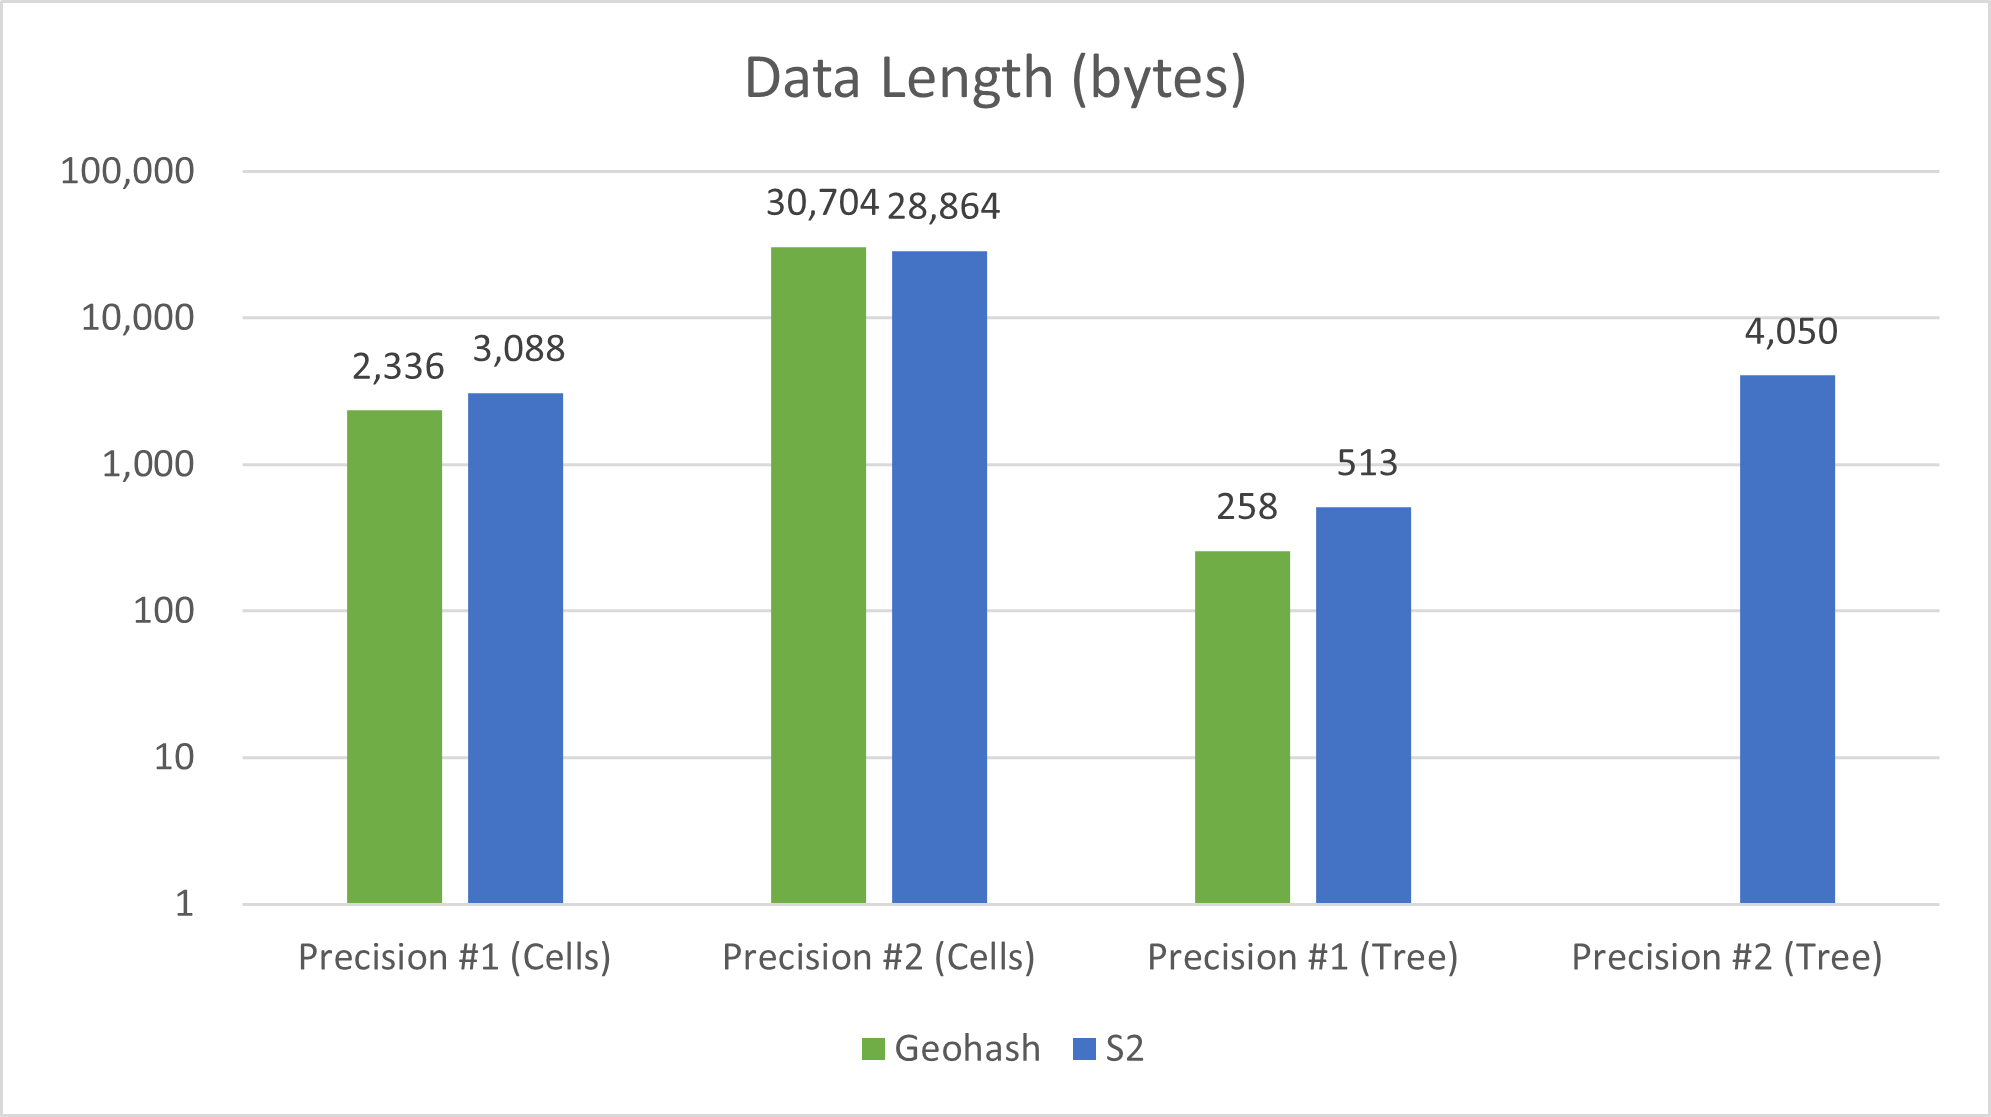
\includegraphics[width=\textwidth]{images/ExperimentRegionsLength.png}
  \caption{Graph showing the sizes of the input data used for adding new regions into the contracts}
  \label{fig:ExperimentRegionsLength}
\end{figure}

\begin{figure}[htb!]
  \centering
  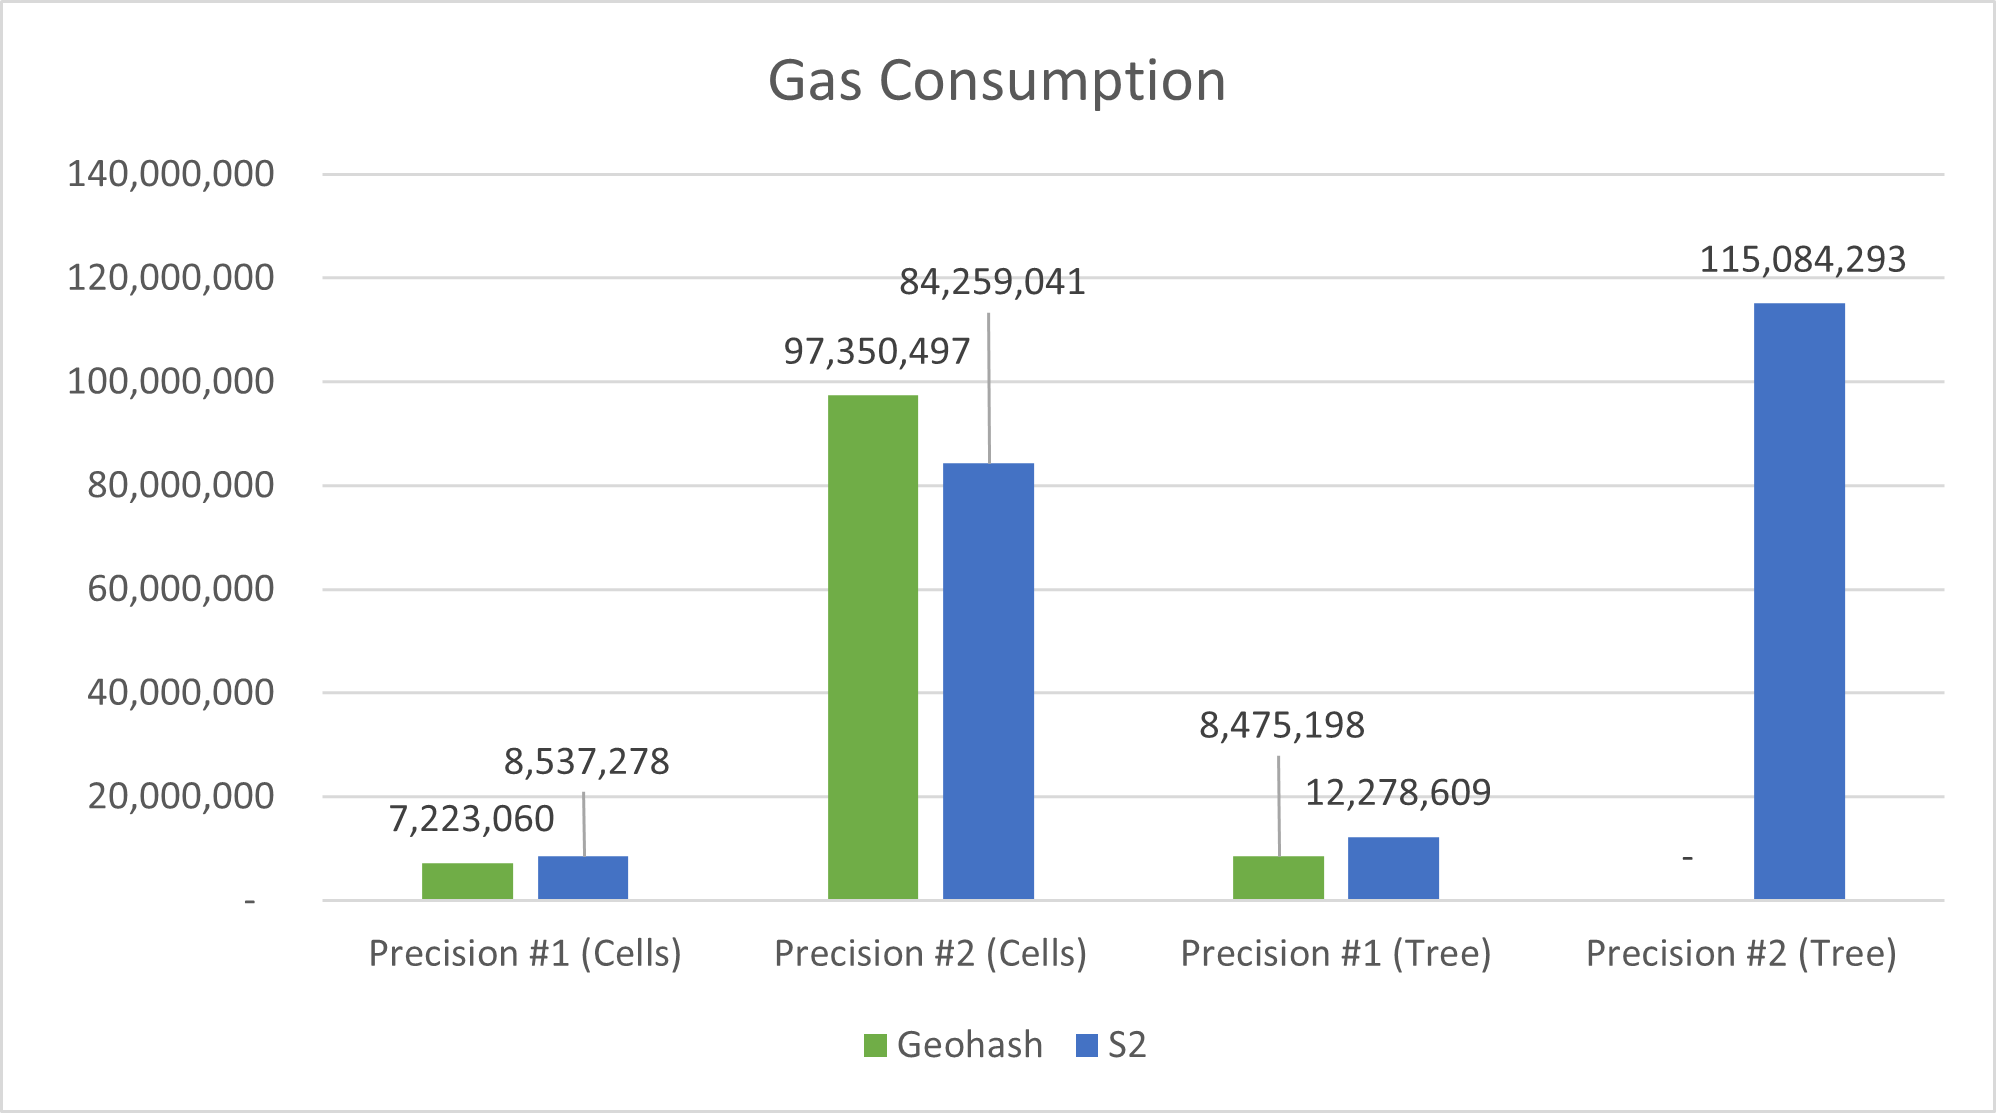
\includegraphics[width=\textwidth]{images/ExperimentRegionsGas.png}
  \caption{Graph showing gas consumption when adding new regions into the contracts}
  \label{fig:ExperimentRegionsGas}
\end{figure}

\begin{figure}[htb!]
  \centering
  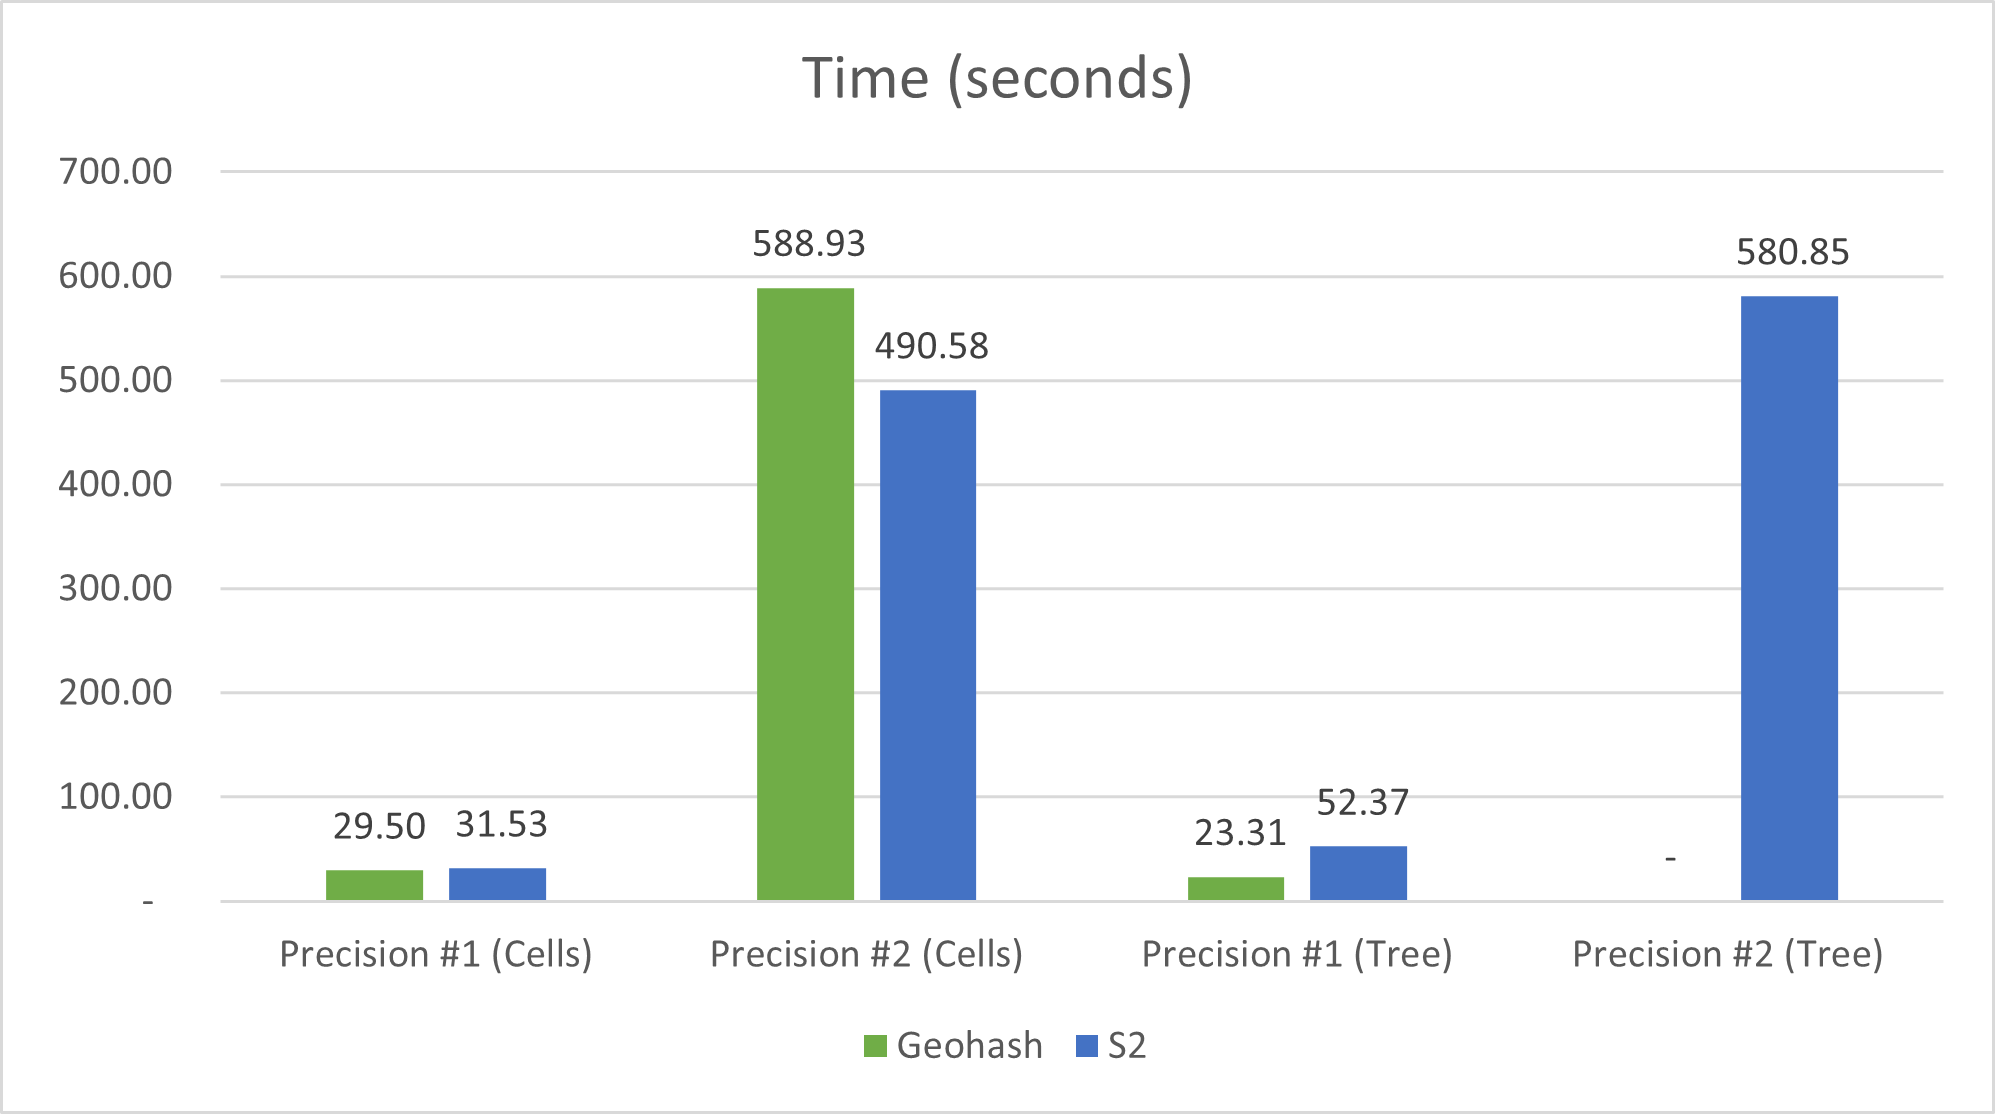
\includegraphics[width=\textwidth]{images/ExperimentRegionsTime.png}
  \caption{Graph showing time spent when adding new regions into the contracts}
  \label{fig:ExperimentRegionsTime}
\end{figure}

\npara Figure \ref{fig:ExperimentRegionsLength} shows the input data lengths of the different regions contracts implementation.
The precision \verb|#|2 of Geohash tree returned an error of \textit{out of gas}, therefore it cannot be included to the result graph.
From the result it can be observed that the sizes of tree-based compressed input data are significantly less than the cell lists.

\npara Figure \ref{fig:ExperimentRegionsGas} shows gas consumption when adding the regions into the Smart Contract.
Despite their significant smaller size of input data, adding data using the trees consumes more gas than using only an array of geocoded cells.
A possible reason is that using Ethereum to expand the tree causes an additional cost of computation.

\npara Figure \ref{fig:ExperimentRegionsTime} shows time spent to add the regions data into the Smart Contract.
It can be observed that in some cases tree-base input data spends more time than cells array but it results in another way in the other cases.
There might be another factor that affects the calculation time in this experiment, however, by the current result data it is difficult to conclude which one is faster.

\begin{figure}[htb!]
  \centering
  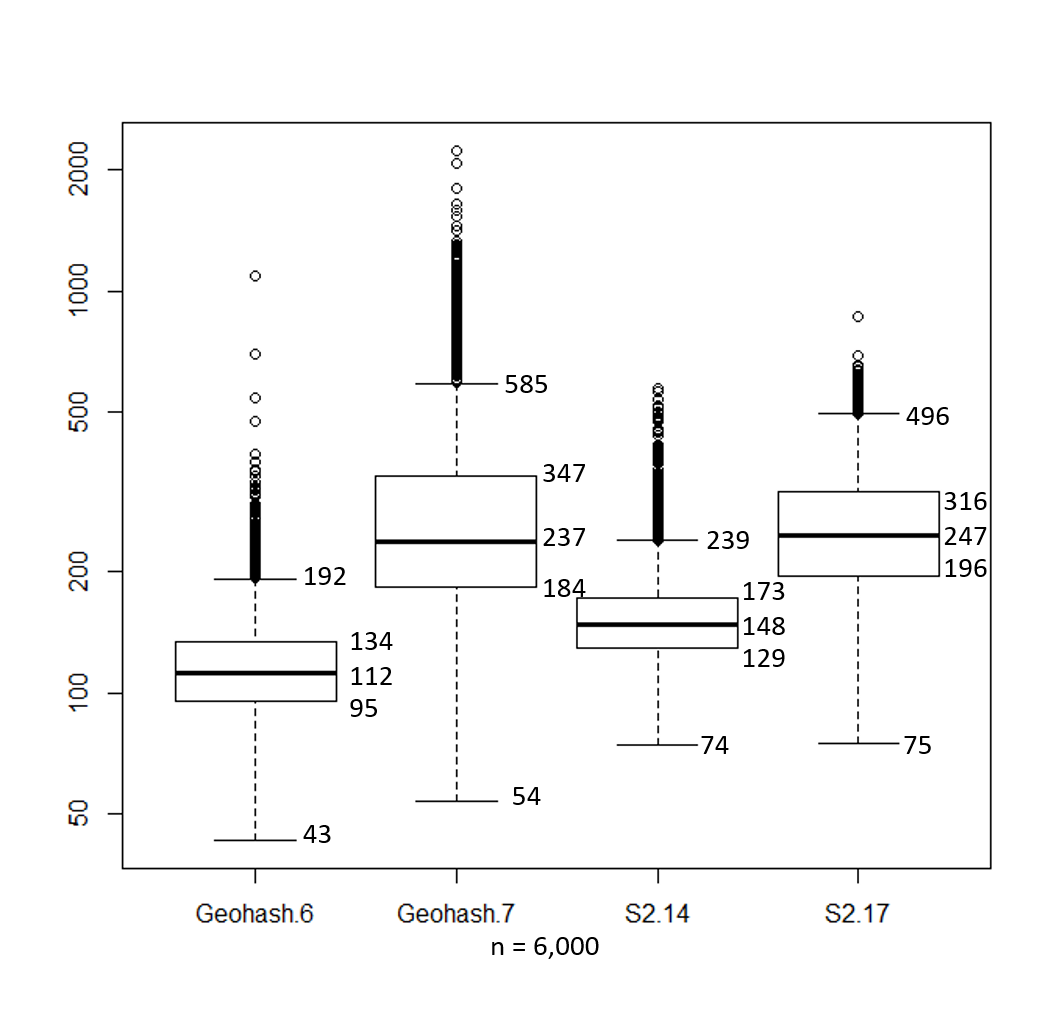
\includegraphics[width=\textwidth]{images/ExperimentQuery.png}
  \caption{Graph showing time spent when querying for a cell in the contracts (in millisecond)}
  \label{fig:ExperimentQuery}
\end{figure}

\npara The last experiment is the query experiment.
This experiment randomly generated 6,000 points in the space and used the same data set to test the query time in the Smart Contracts based on Geohash and S2.
In these 6,000 points, 5,000 of them are belong to an existing region in the Smart Contracts, the other 1,000 are the points that do not fall into any region.
Figure \ref{fig:ExperimentQuery} shows a boxplot of the experiment results.
From the results, it can be observed that in the similar level, querying for a cell in Geohash is slightly faster than S2.
The reason can be that one level of a Geohash cell requires 5 bits of data while S2 requires 2 bits.
For this reason, to query for a cell over the data, Geohash requires 7 iterations to check across all the levels and S2 requires up to 32 iterations to check.

\subsection*{Mining Performance of the Devices in the System}

\begin{figure}[htb!]
  \centering
  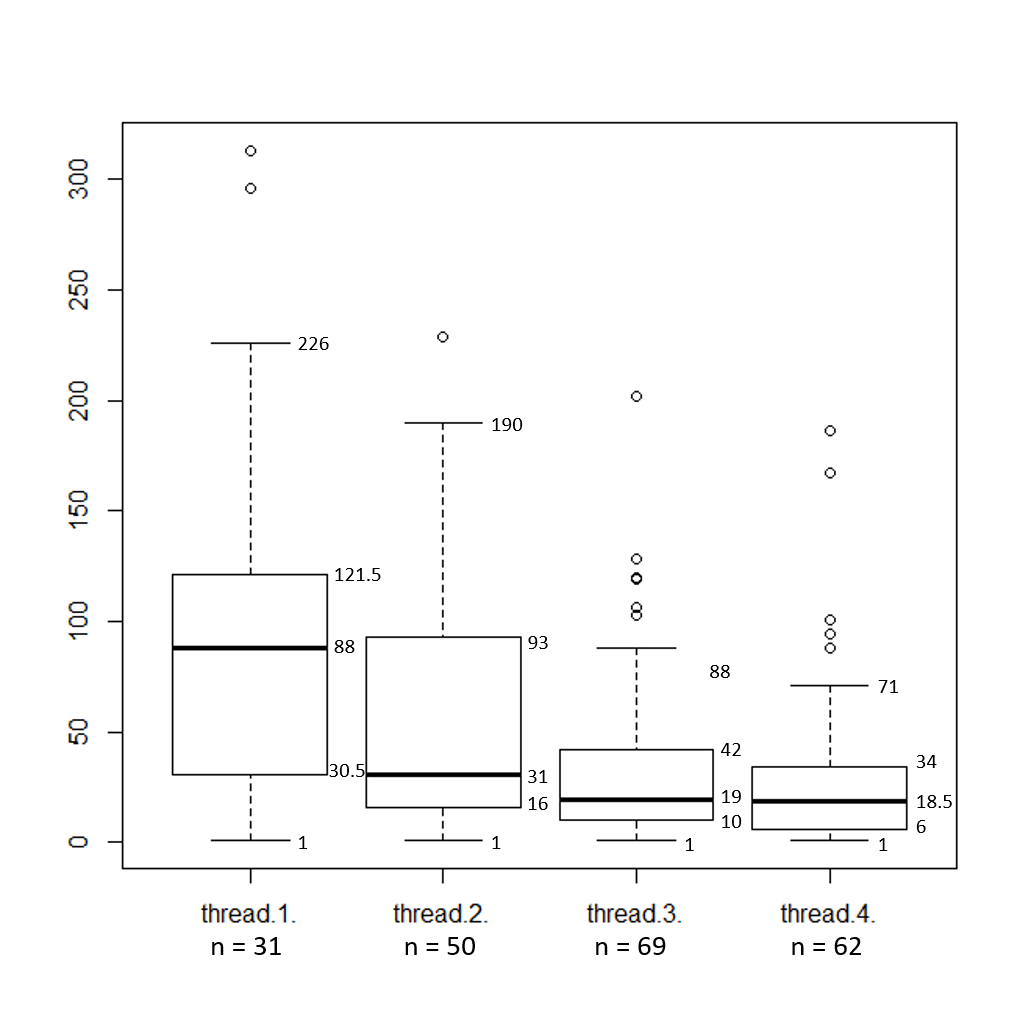
\includegraphics[width=\textwidth]{images/ExperimentMining.png}
  \caption{Graph showing time spent when mining a new block into the chain (in second)}
  \label{fig:ExperimentMining}
\end{figure}

\npara This experiment was designed to compare the possibility and performance of the Ethereum nodes using IoT devices when mining a new block to the chain.
It compares a personal computer of 4-core \hyperref[Acronym-CPU]{CPU} and a Raspberry Pi which is used as a fog device.
However, due to hardware limitation, the Raspberry Pi did not manage to mine any block.
Instead, it returned an out of memory error and halted the Ethereum client.
For this reason, despite the fact that Raspberry Pi can be a node in Ethereum network and can submit the transactions, it cannot be a miner to publish the chain.
A possible solution to this issue is to modify the implementation of the Ethereum network to use a different consensus algorithm, whose default is Proof-of-Work, to be the Proof-of-Authority algorithm\footnote{\hyperlink{https://ethereum.stackexchange.com/questions/24955/geth-mining-on-32bits-host-raspberry-pi-memory-error}{\code{https://ethereum.stackexchange.com/questions/24955/\newline
geth-mining-on-32bits-host-raspberry-pi-memory-error}}}.
However, this experiment continued to measure the mining time using only the personal computer running on the different thread numbers, keeping the default consensus algorithm which is Proof-of-Work.
Figure \ref{fig:ExperimentMining} shows the results of the experiment.
As expected, using more thread tends to spend less time to mine a block into the chain.
The mining time indicates time needed to publish a transaction into the network.
Hence, from the results it can take up to minutes for a change in the Smart Contract to be propagated over the network.
\newpage

\section{Experiment: Deployment and Scenario} \label{Results-Deployment}

\npara This sections describes the results and related discussions after having deployed the proposed architecture into the real \hyperref[Acronym-IoT]{IoT} devices.

\subsection*{Fog Layer}

\begin{figure}[hbt!]
  \centering
  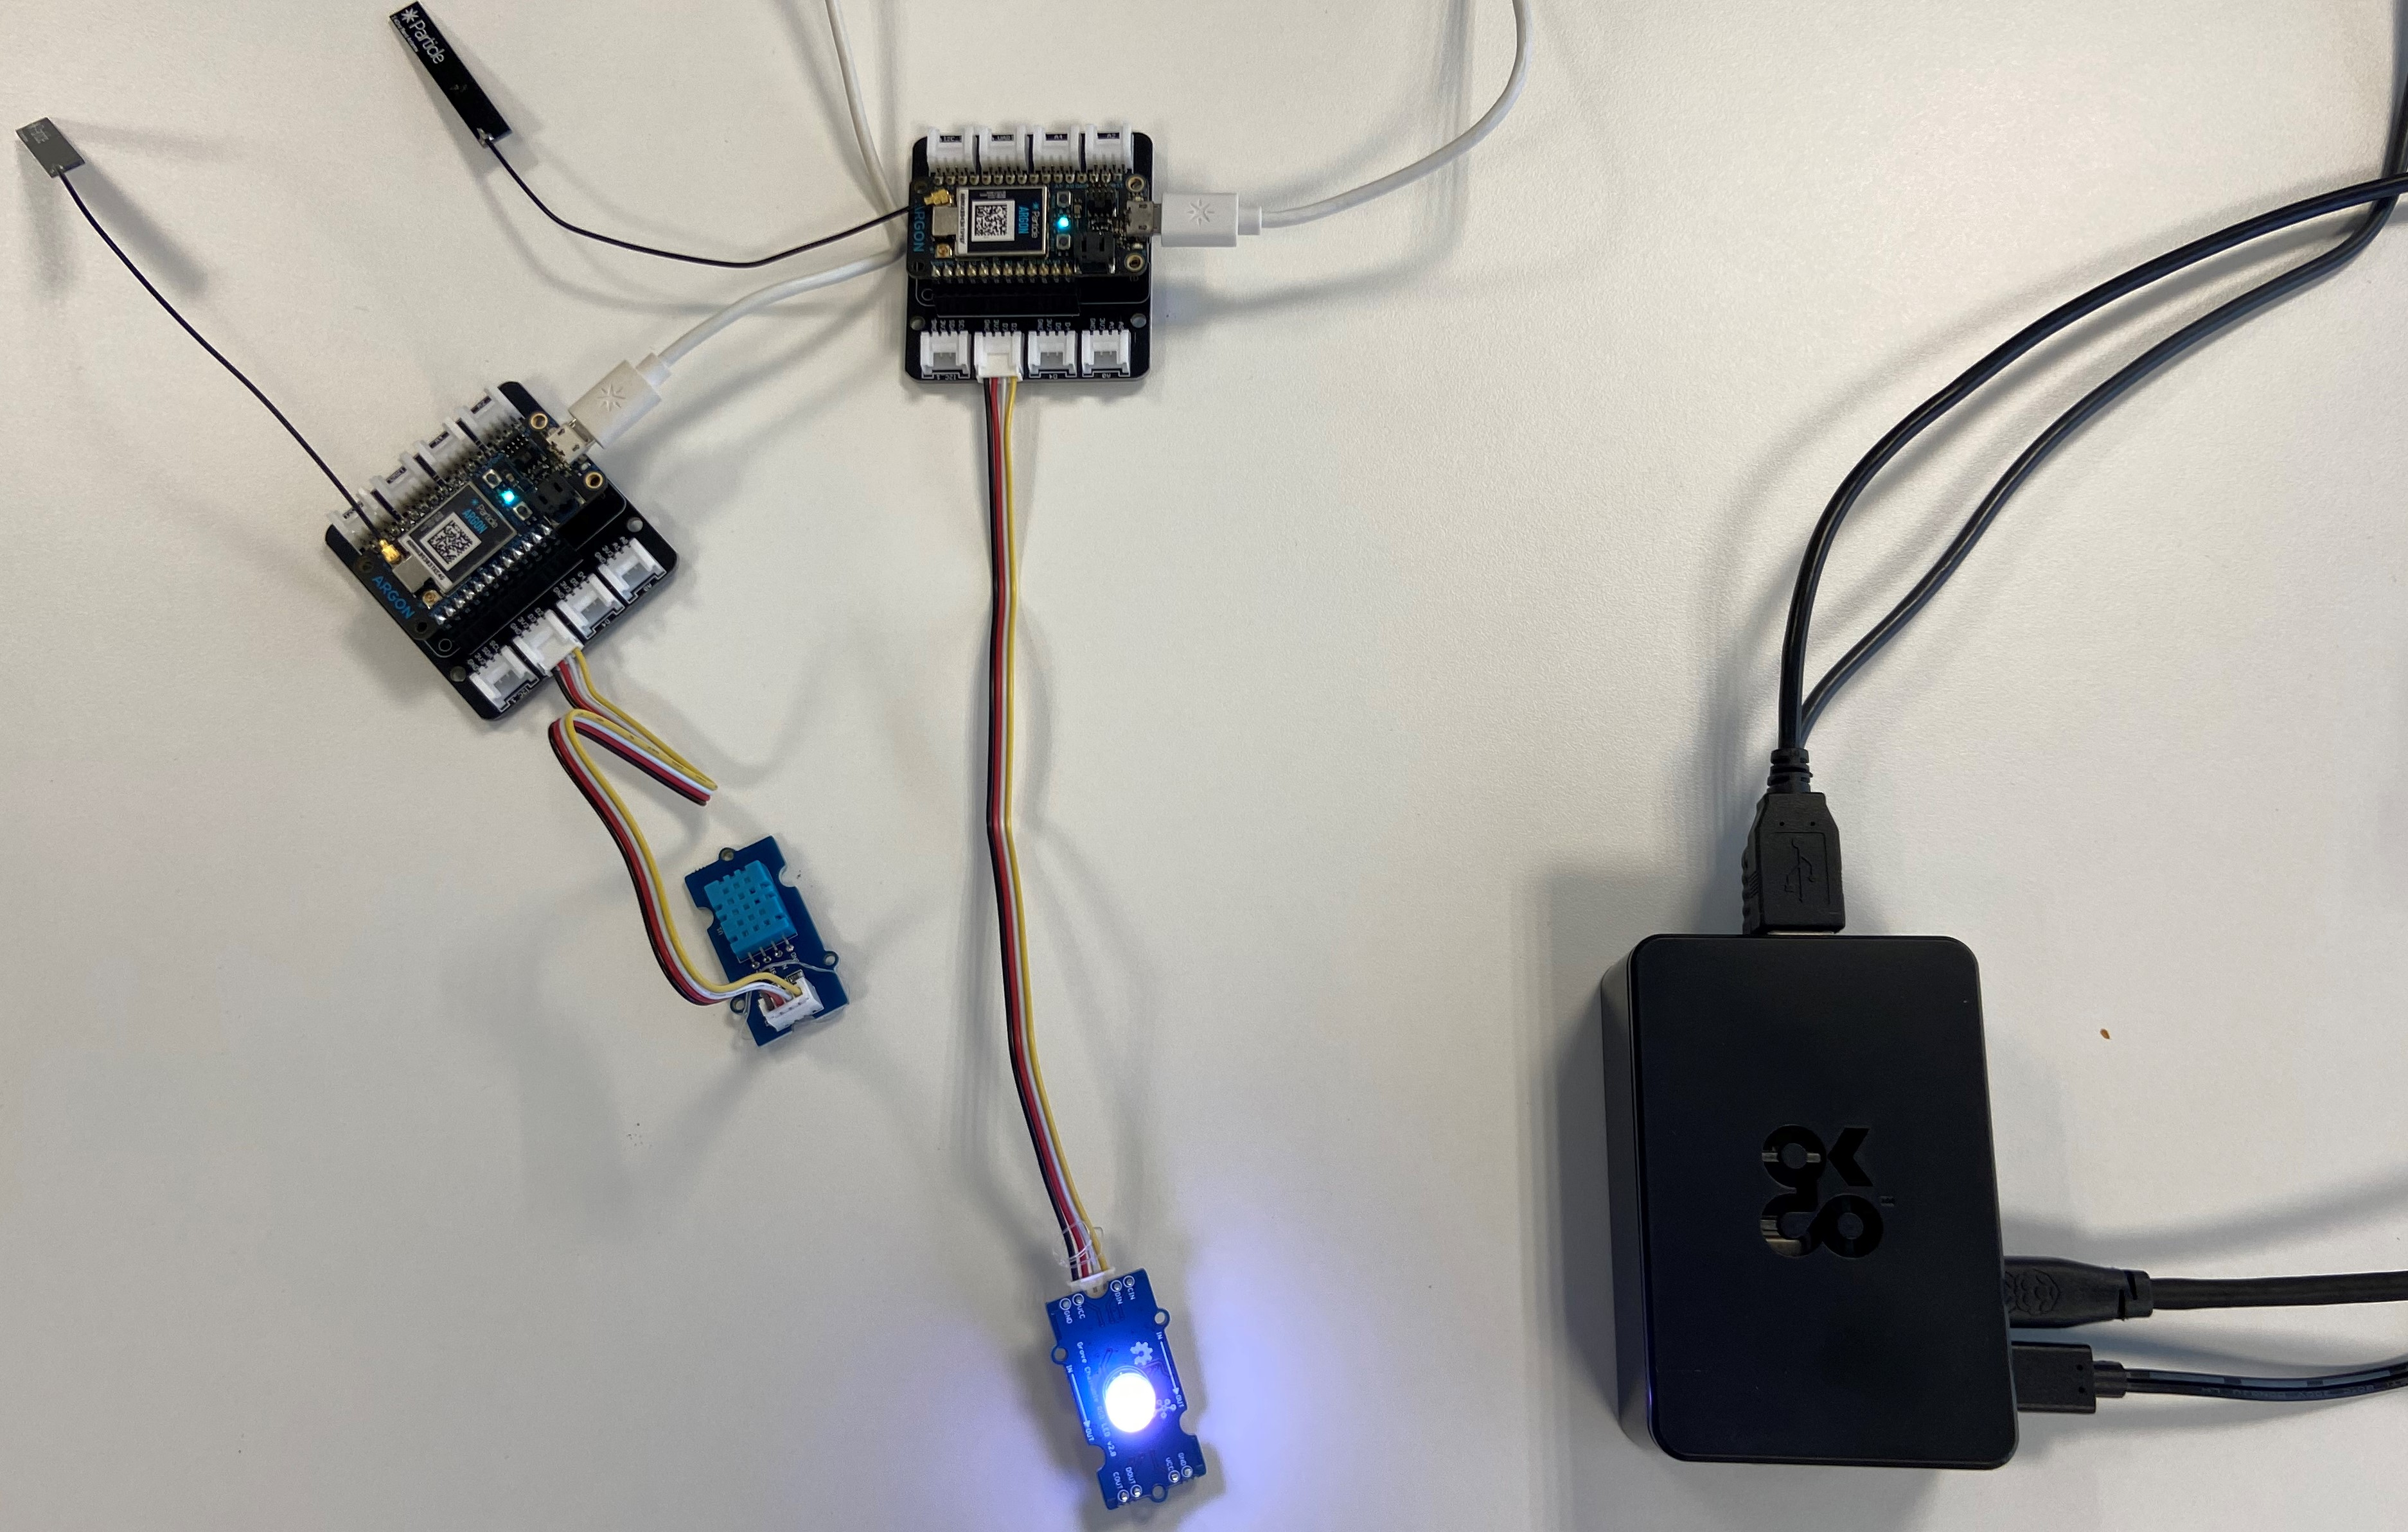
\includegraphics[width=\textwidth]{images/ScenarioBlue.jpg}
  \caption{The instalment of test scenario: edge service provider, edge service consumer, fog Raspberry Pi}
  \label{fig:ScenarioBlue}
\end{figure}

\npara The \hyperref[Acronym-API]{API}s and a Geth client were installed into a Raspberry Pi 4.
After using the API to interact with the Smart Contracts, it showed that the Raspberry Pi 4 has enough potential to serve as an \hyperref[Acronym-API]{API} and run an Ethereum node at the same time.
The Raspberry Pi, whose operating system is based on Linux, is also able to run another service, including \hyperref[Acronym-SSH]{SSH}, which allows a remote access to the device.
Hence, it is not necessary to be physically with the node in order to maintain, update or configure it.
The shell script\footnote{GitHub repository: \url{https://github.com/ponlawat-w/uji_mt-raspi_scripts}} enables Raspberry Pi to run the \hyperref[Acronym-API]{API} and Geth client as a service, therefore it is simpler for the administrator to access the device via \hyperref[Acronym-SSH]{SSH} and execute the service command in order to start, stop the service, as well as diagnose it when there is a problem.
The Smart Contracts allowed the devices to register themselves with their \hyperref[Acronym-IP]{IP} address information.
Once it is added into the Blockchain, another node can also see the list of the registered fog nodes and their \hyperref[Acronym-IP]{IP} addresses, so that they can use the \hyperref[Acronym-IP]{IP} address as a \hyperref[Acronym-URL]{URL} base for the \hyperref[Acronym-API]{API}.

\npara However, in this test scenario, the registered \hyperref[Acronym-IP]{IP} addresses is in the same \hyperref[Acronym-LAN]{LAN} network.
In practice, fog node can be installed in a different area which uses a different internet network.
It might be necessary to consider using another service to forward device \hyperref[Acronym-IP]{IP} address or using a \hyperref[Acronym-VPN]{VPN} to let the device be accessible from outside.

\npara Figure \ref{fig:ScenarioBlue} shows the instalment of this test experiment.
The Raspberry Pi who acts as a fog node is located as a black box in the right side of the image.

\subsection*{Edge Layer}

\begin{figure}[hbt!]
  \centering
  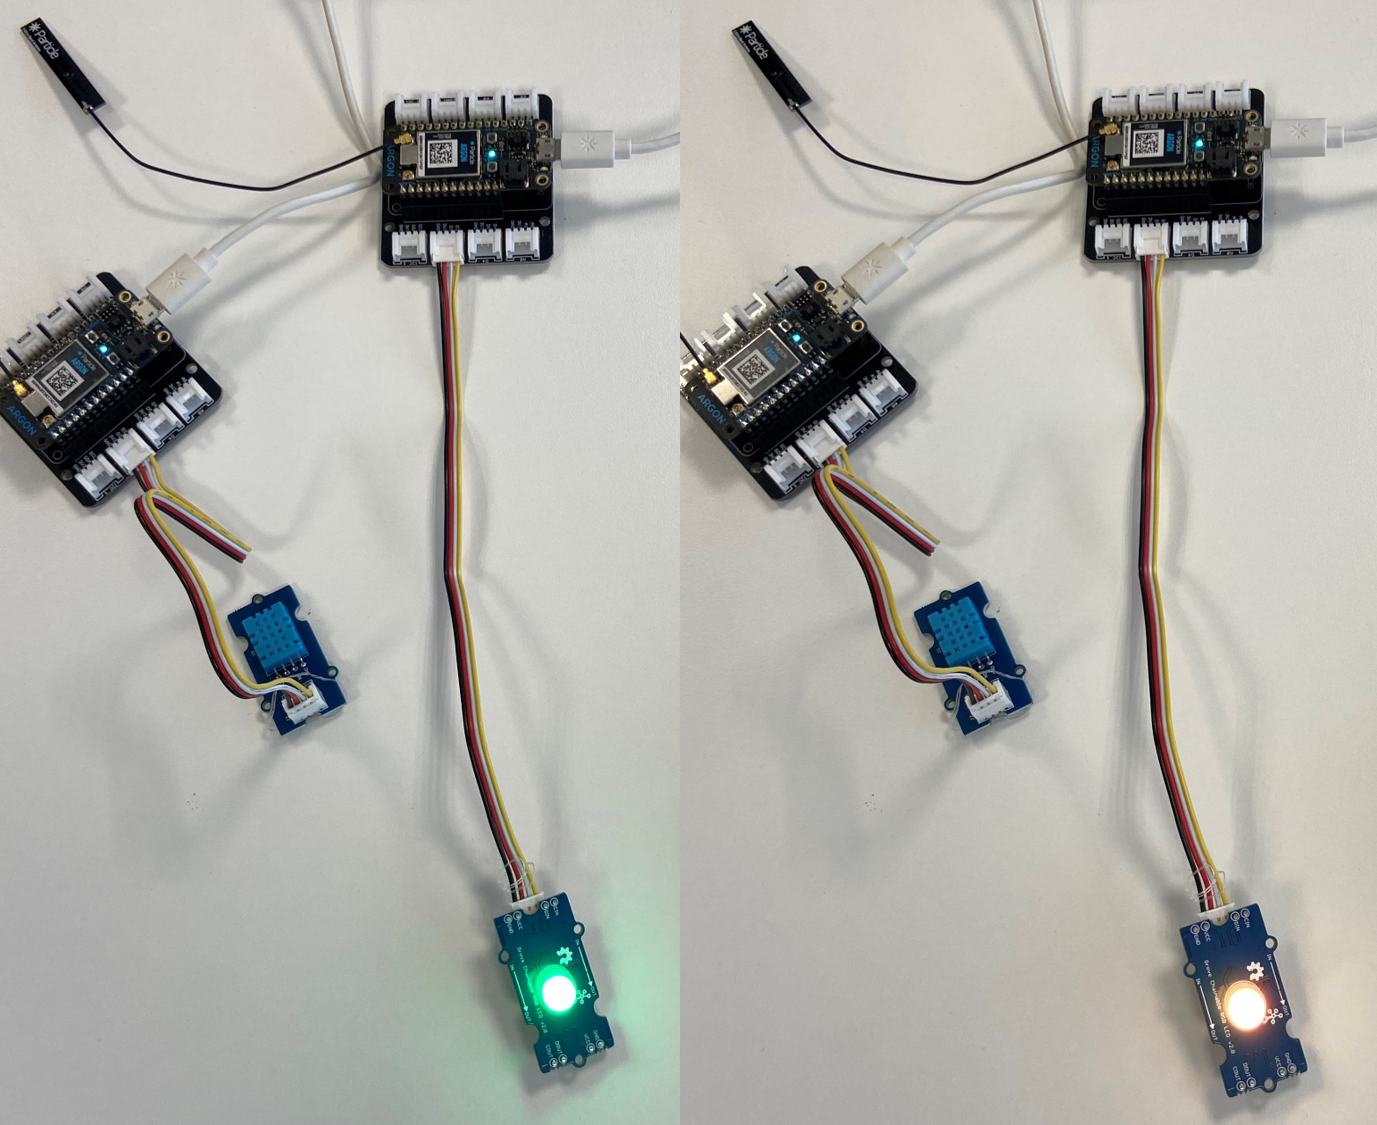
\includegraphics[width=\textwidth]{images/ScenarioGreenOrange.png}
  \caption{The service consumer status \hyperref[Acronym-LED]{LED} shows in green (trust) and orange (not trust)}
  \label{fig:ScenarioGreenOrange}
\end{figure}

\npara In the test scenario, the edge service provider was attached to a temperature and humidity sensor, and exposed the services into its device registration data.
However, due to lack of equipment, it was unfortunately not able to equip a \hyperref[Acronym-GPS]{GPS} module or any positioning module to it.
Thus, the device's position had to be simulated and manually set by the user, which is not supposed to be the case in the practical implementation.

\npara After the device had been switched on, it was able to received an Ethereum address and private key from the user, and register itself to the Smart Contracts through the fog \hyperref[Acronym-API]{API}.
To send the transaction, the device managed to sign a transaction and submit to the fog \hyperref[Acronym-API]{API}.
Using an \hyperref[Acronym-HTTP]{HTTP} caller application in the personal computer (in this case \textit{Postman}), it was able to communicate with the edge device through its \hyperref[Acronym-API]{API} served on the exposed \hyperref[Acronym-IP]{IP} address.
The \hyperref[Acronym-IP]{IP} address of the device can be discovered by query in the contract via the fog \hyperref[Acronym-API]{API}.
It was also able to query for the reputation value using fog \hyperref[Acronym-API]{API} and establish a new connection to consume the service.
The service provider returned correct values of the service, and parallelly sent the observed data to the fog node as defined in the architecture.
Finally, after finishing the service consumption, the user sent a feedback to the fog node, which was later calculated (or random in this work) to be a new updated reputation value of the service, and updated in the Smart Contracts.
When a user query again for the reputation value, the smart contract returns the updated value as expected.

\npara The experiment was extended by changing the service consumption from being manual to automatic by using another edge device.
The service consumer device is equipped with an \hyperref[Acronym-LED]{LED} that can emit light in red-green-blue shades of colour.
The device was programmed to expose its communication status via \hyperref[Acronym-LED]{LED}, which is
  red when it cannot connect to the fog node,
  orange when there is no any satisfying reputed service provider in the area,
  blue when it is establishing a new connection with a service provider,
  and green when it is correctly consuming the service.
The result shows that the service consumer worked correctly.
It emitted an orange signal when the queried area has no service providers whose reputation value satisfied the threshold, and it emitted a green one when there was a service provider that was trusted and selected to establish a new connection as shown in Figure \ref{fig:ScenarioGreenOrange}.
